\documentclass[a4paper,twoside,DIV15,BCOR12mm]{scrbook}

\usepackage{mathe}
\usepackage{saetze-veraart}
\usepackage{faktor}
\usepackage{enumerate}
\usepackage{tikz}
\usepackage{german}
\usepackage{wrapfig}
\usepackage{ziffer}

%\usepackage{lmodern}

% \usepackage{remreset}
% \makeatletter
% \@removefromreset{section}{chapter}
% \makeatother

\newcommand{\cX}{\mathcal X}
\newcommand{\cM}{\mathcal M}
\newcommand{\cA}{\mathcal A}
\newcommand{\cV}{\mathcal V}
\newcommand{\cF}{\mathcal F}
\newcommand{\borel}{{\mathfrak B}}
\newcommand{\unisucceq}{\succeq_{\text{uni}}}
\newcommand{\mvsucceq}{\succeq_{\text{mv}}}
\newcommand{\monsucceq}{\succeq_{\text{mon}}}
\newcommand{\dickerkringel}{\bullet}

\DeclareMathOperator{\ARA}{ARA}
\DeclareMathOperator{\RRA}{RRA}
\DeclareMathOperator{\Var}{Var}
\DeclareMathOperator{\Cov}{Cov}
\DeclareMathOperator{\VatR}{V@R}
\DeclareMathOperator{\AVatR}{AV@R}

\author{Die Mitarbeiter von \url{http://mitschriebwiki.nomeata.de/}}
\title{Finanzmathematik I}
\makeindex

\begin{document}
\maketitle
 
\newenvironment{enuma}{%
\begin{enumerate}[\hspace{1em}a)]%
}{%
\end{enumerate}%
}

\newenvironment{enumi}{%
\begin{enumerate}[\hspace{1em}i)]%
}{%
\end{enumerate}%
}

\setcounter{secnumdepth}{-1}
%\renewcommand{\thechapter}{\arabic{chapter}}
%\chapter{Inhaltsverzeichnis}
%\stepcounter{chapter}
%\renewcommand{\tocname}{bla}
%\addcontentsline{toc}{chapter}{\protect\numberline {\thechapter}Inhaltsverzeichnis}
\addcontentsline{toc}{chapter}{Inhaltsverzeichnis}
\tableofcontents

 % Vorwort

\chapter{Vorwort}
\setcounter{secnumdepth}{2}
%\addcontentsline{toc}{chapter}{Vorwort}

\section*{Über dieses Skriptum}
Dies ist ein Mitschrieb der Vorlesung \glqq Finanzmathematik I\grqq\ von Dr. Veraart im
Wintersemester 08/09 an der Universität Karlsruhe (TH).
% Die Mitschriebe der Vorlesung werden mit ausdrücklicher Genehmigung von Dr. Veraart hier veröffentlicht,
Dr. Veraart ist für  den Inhalt nicht verantwortlich.
\section*{Wer}
Gestartet wurde das Projekt von Joachim Breitner.
%Weiter haben Felix Wellen und Michael Walter beim Mitschreiben geholfen.

\section*{Wo}
Alle Kapitel inklusive \LaTeX-Quellen können unter \url{http://mitschriebwiki.nomeata.de} abgerufen werden.
Dort ist ein von Joachim Breitner programmiertes \emph{Wiki}, basierend auf \url{http://latexki.nomeata.de} installiert. 
Das heißt, jeder kann Fehler nachbessern und sich an der Entwicklung
beteiligen. Auf Wunsch ist auch ein Zugang über \emph{Subversion} möglich.

%\setcounter{chapter}{0}
%\renewcommand{\thesection}{{\rm\bfseries §}\arabic{section}}
\renewcommand{\thesection}{\arabic{chapter}.\arabic{section}}
\renewcommand{\thechapter}{\Roman{chapter}}

\chapter{Einführung in die Theorie der Finanzmärkte}

\section{Präferenzen}

Modelle, die den Finanzmarkt beschreiben, müssen stochastisch sein, um \emph{Risiko} adäquat modellieren zu können.

Ein \emph{Markt} ist ein Ort, an dem Güter und Dienstleistungen von \emph{Agenten} ausgetauscht werden, deren Handlungen durch ihre \emph{Präferenzen} bestimmt werden.

Sei $\cX$ eine nichtleere Menge. $x\in\cX$ bezeichnet die Wahlmöglichkeit eines Agenten.

\begin{definition}
Eine binäre Relation $\succeq \subseteq \cX \times \cX$ heißt \emph{Präferenzenrelation}\index{Präferenzenrelation}, falls sie
\begin{itemize}
\item transitiv ist, also $\forall x,y,z \in\cX$: $x\succeq y$, $y\succeq z \implies x\succeq z$
\item vollständig ist, also $\forall x,y\in \cX$: $x\succeq y$ oder $y\succeq x$
\end{itemize}
Falls $x\succeq y$ und $y\succeq x$ schreiben wir $x\sim y$ (\emph{Indifferenzrelation}\index{Indifferenzrelation}). Für $x\succeq y$ und $y\not\succeq x$, dann schreiben wir $x\succ y$.
\end{definition}

\begin{beispiel}
$\cX=\MdR$, $x\succeq y \iff x\ge y$
\end{beispiel}

\begin{definition}
Eine \emph{numerische Repräsentation}\index{numerische Repräsentation} einer Präferenzordnung $\succeq$ ist eine Funktion $U:\cX\to R$, so dass $x\succeq y \iff U(x) \ge U(y)$.
\end{definition}

\begin{bemerkung}
Eine numerische Repräsentation ist nicht eindeutig: Sei $f$ eine streng monoton wachsende Funktion. Dann ist $\tilde U(x) \da f(U(x))$ auch eine numerische Repräsentation.
\end{bemerkung}

\begin{beispiel}
Sei $\succeq$ die lexikographische Ordnung auf $\cX \da [0,1]\times[0,1]$, also\[(x_1,y_1)\succ (x_2,y_2) \iff x_1 > x_2 \text{ oder } x_1 = x_2 \text{ und } y_1 > y_2.\] Für $\succeq$ gibt es keine numerische Repräsentation.
\end{beispiel}

\begin{definition}
Sei $\succeq$ Präferenzenrelation auf $\cX$. Eine Teilmenge $\mathcal Z\subseteq \mathcal X$ heißt \emph{dicht}\index{dicht} in $\cX$ (bezüglich $\succeq$), falls für alle $x,y\in\cX$ mit $x\succ y$ ein $z\in\mathcal Z$ gibt, so dass $x\succeq z \succeq y$.
\end{definition}

\begin{beispiel}
$\cX = \MdR$, $\mathcal Z=\MdQ$, $\succeq = \ge$.
\end{beispiel}

\begin{satz}
Für die Existenz einer numerischen Repräsentation einer Präferenzenrelation $\succeq$ ist es notwendig und hinreichend, dass $\cX$ eine abzählbare Teilmenge $\mathcal Z$ enthält, die dicht in $\cX$ liegt.

Insbesondere hat für abzählbare $\cX$ jede Präferenzenrelation eine numerische Repräsentation.
\end{satz}

\begin{beweis}
siehe Föllmer \& Schied, Beweis von Theorem 2.6
\end{beweis}

\subsection{Von Neumann-Morgenstern-Repräsentation}

Im Folgenden betrachten wir das Konzept des erwarteten Nutzens.

Es seien alle Wahlmöglichkeiten eines Agenten durch Wahrscheinlichkeitsverteilungen auf einer vorgegebenen Menge von Szenarien gegeben. Sei $(S,\mathfrak S)$ ein messbarer Raum und $M_1(S,\mathfrak S)$ die Menge aller Wahrscheinlichkeitsverteilungen auf $(S,\mathfrak S)$. Wir betrachten eine Teilmenge $M\subseteq M_1(S,\mathfrak S)$. Wir nehmen an, dass $M$ konvex ist, das heißt für alle $\mu, \nu\in M$ und alle $\alpha\in[0,1]$ ist $\alpha\mu + (1-\alpha)\nu \in M$. Die Elemente von $M$ werden auch \emph{Lotterien}\index{Lotterie} genannt.

\begin{definition}
\label{def.1.1.9}
Eine numerische Repräsentation einer Präferenzordnung wird \emph{von-Neumann-Morgenstern-Re\-prä\-sen\-tat\-ion}\index{von-Neumann-Morgenstern-Repräsentation} genannt, falls sie sich darstellen lässt als:
\[ U(\mu) = \int u(x)\mu(dx)\ \forall \mu\in M\]
wobei $u$ eine reelle Funktion auf $S$ ist.
\end{definition}

Wir werden später die Funktion $u$, wenn sie gewisse Voraussetzungen erfüllt, Nutzenfunktion nennen.

Wir betrachten beispielsweise eine Zufallsvariable $X$ auf einem Wahrscheinlichkeitsraum $(\Omega, \F, P)$, die die Auszahlung einer Anlagemöglichkeit angibt. 

Ist etwa $S\subseteq \MdR$, $\mathfrak S = \borel\footnote{Borelsche $\sigma$-Algebra}$, dann bezeichnet das Integral in der Definition \ref{def.1.1.9} den Erwartungswert von $u(X)$, wobei $u$ messbar (später stetig) sei und $X$ die Verteilung 
\[\mu(B) \da P_X(B)=P(X^{-1}(B)) \ \forall B\in\borel \]
besitzt.

Wann existiert eine von-Neumann-Morgenstern-Repräsentation?

Sei $M$ die Menge aller Wahrscheinlichkeitsmaße $\mu$ auf $S$, die sich als Linearkombination $\mu=\sum_{i=1}^N \alpha_i\delta_{x_i}$ von $x_1,\ldots,x_N\in S$ mit Koeffizienten $\alpha_1,\ldots,\alpha_N\in (0,1]$ darstellen lässt. Das Dirac-Maß ist dabei definiert als
\[ \delta_x(A) = 
\begin{cases}
1,&x\in A\\
0,&\text{sonst}
\end{cases}\]

Dann existiert eine von-Neumann-Morgenstern-Repräsentation, falls $\succeq$ die folgenden Eigenschaften hat:
\begin{itemize}
\item \emph{Unabhängigkeitseigenschaft}\index{Unabhängigkeitseigenschaft}: Für alle $\mu,\nu\in M$ mit $\mu\succ \nu$, alle $\alpha \in(0,1]$ und beliebige $\lambda\in M$ gilt:
\[ \alpha \mu + (1-\alpha) \lambda \succ \alpha \nu + (1-\alpha)\lambda \]
das heißt, dass die Präferenz $\mu\succ \nu$ in jeder Konvexkombination erhalten bleibt, unabhängig von der zusätzlichen Lotterie $\lambda$.

\item \emph{Archimedeseigenschaft}\index{Archimedeseigenschaft}, Stetigkeitseigenschaft: Zu jedem Tripel $\mu\succ \lambda  \succ \nu$ existieren Konstanten $\alpha,\beta\in(0,1)$, so dass gilt:
\[
\alpha\mu + (1-\alpha)\nu \succ \lambda \succ \beta \mu + (1-\beta)\nu
\]
\end{itemize}

Falls $S$ eine endliche Menge ist, haben alle Maße die obige Darstellung als Konvexkombination von Dirac-Maßen.

Im allgemeinen Fall benötigt man für die Existenz einer von-Neumann-Morgenstern-Repräsentation neben der Unabhängigkeitseigenschaft und der Archimedeseigenschaft noch eine weitere Eigenschaft von $\succeq$ („sure thing principle“).

Für $\mu,\nu \in M$ und $A$ mit $\mu(A)=1$ gilt:
\begin{align*}
(\forall x\in A:\delta_x\succ \nu) &\implies \mu \succ \nu \\
(\forall x\in A:\nu \succ \delta_x) &\implies \nu \succ \mu
\end{align*}

Beweise siehe Föllmer und Schied, Kapitel 2.2.

\subsection{Risikoaversion}

Wir betrachten Anlagemöglichkeiten (z.B. Aktien), deren Verteilung der Auszahlung zu einem festen Zeitpunkt bekannt ist. Die Verteilung wird als Wahrscheinlichkeitsverteilung auf einem Intervall $S\subseteq \MdR$ angenommen. $\cM$ sei die Menge aller Borel-Wahrscheinlichkeitsmaße auf $S$. Wir nehmen an, dass $\cM$ konvex ist und alle Punktmaße $\delta_x$ für $x\in S$ enthält. Wir nehmen an, dass für alle $\mu\in\cM$ die Erwartung 
\[
m(\mu) \da \int x \mu (dx) \in \MdR
\]
wohldefiniert ist.

\begin{definition}
\begin{itemize}
\item Eine Präferenzrelation $\succeq$ auf $\cM$ wird \emph{monoton}\index{monotone Präferenzrelation} genannt, wenn $x>y$ impliziert, dass $\delta_x \succ \delta_y$.
\item Eine Präferenzrelation $\succeq$ wird \emph{risikoavers}\index{risikoaverse Präferenzrelation} genannt, falls für alle $\mu\in\cM$ mit $\mu \ne \delta_{m(\mu)}$ gilt, dass $\delta_{m(\mu)} \succ \mu$.
\end{itemize}
\end{definition}

\begin{satz}
Eine Präferenzrelation $\succeq$ ist 
\begin{enumerate}
\item monoton, genau dann wenn $u$ streng monoton wachsend ist.
\item risikoavers, genau dann wenn $u$ streng konkav ist.
\end{enumerate}
\end{satz}

\begin{beweis}
\begin{enumerate}
\item Sei $x>y$. Monotonie ist äquivalent zu $u(x)=\int u(s) \delta_x(ds) = U(\delta_x) > U(\delta_y) = u(y)$.
\item Sei $\succeq$ risikoavers. Dann gilt für verschiedene $x,y\in S$ und $\alpha \in (0,1)$
\[
\delta_{\alpha x + (1-\alpha) y} \succ \alpha \delta_x + (1-\alpha)\delta_y
\implies
u(\alpha x + (1-\alpha ) y) > \alpha u(x) + (1-\alpha) u(y)
\]
also ist $u$ streng konkav.

Sei $u$ streng konkav. Risikoaversion folgt aus der Jensen-Ungleichung, da
\begin{align*}
U(\delta_{m(\mu)}) = u(m(\mu)) = u\Big(\int x \mu (dx)\Big) \ge \int u(x) \mu(dx) = U(\mu)
\end{align*}
Es gilt Gleichheit für $\mu = \delta_{m(\mu)}$.
\end{enumerate}
\end{beweis}

\begin{definition}
Eine Funktion $u:S\to\MdR$ heißt \emph{Nutzenfunktion}\index{Nutzenfunktion}, falls sie streng monoton wachsend, streng konkav und stetig\footnote{Wobei nur die Stetigkeit auf dem Rand von $S$ extra zu fordern wäre.} auf $S$ ist.
\end{definition}

Im Folgenden betrachten wir nur noch Präferenzrelationen $\succeq$ auf $\cM$, die eine von-Neumann-Morgenstern-Repräsentation $U(\mu) = \int u d \mu$ mit einer Nutzenfunktion $u:S\to\MdR$ haben. 

Die Anwendung des Zwischenwertsatzes auf die streng monoton wachsende, stetige Funktion $u$ liefert für jedes $\mu\in\cM$ die Existenz einer eindeutigen reelen Zahl $c(\mu)\in S$ mit
\[u(c(\mu)) = U(\mu) = \int ud\mu\]
Dann gilt $\delta_{c(\mu)} \sim \mu$, das heißt der Agent ist indifferent zwischen der sicheren Auszahlung $c(\mu)$ und der Lotterie $\mu$. 

\begin{definition}
Das \emph{Sicherheitsäquivalent}\index{Sicherheitsäquivalent} einer Lotterie $\mu\in \cM$ ist die reele Zahl $c(\mu)\in S$, die 
\begin{align*}
u(c(\mu)) = U(\mu) = \int ud\mu
\end{align*}
löst.

Die \emph{Risikoprämie}\index{Risikoprämie} von $\mu$ ist definiert als $\rho(\mu)\da m(\mu) - c(\mu)$.
\end{definition}

Risikoaversion impliziert über die Jensen-Ungleichung, dass $c(\mu) \le m(\mu)$ gilt, und dass Gleichheit genau dann gilt, wenn $\mu = \delta_{m(\mu)}$.

\begin{beispiel}
Siehe St. Petersburg-Paradox, Übungsblatt 1
\end{beispiel}

\begin{beispiel}[Beispiele für Nutzenfunktionen]
\begin{itemize}
\item $u(x) = - e^{-\gamma x}$, wobei $\gamma>0$ der Koeffizient der absoluten Risikoaversion ist. Diese Funktion wird CARA (“constant absolute risk aversion”) genannt.
\item $u(x) = 
\begin{cases}
\frac{x^{1-R}}{1-R}, & x > 0 \\
-\infty, & x \le 0
\end{cases}$, wobei $R>0$, $R\ne 1$ der Koeffizient der relativen Risikoaversion ist. Diese Funktion wird CRRA (“constant relative risk aversion”) genannt.
\item $u(x) = 
\begin{cases}
\log x, & x > 0 \\
-\infty, & x \le 0
\end{cases}$ ist CRRA-Nutzenfunktionen für $R=1$.
\item Die Funktion $u(x) = x - \frac\varepsilon2x^2$, $\varepsilon>0$, ist konkav, aber nicht monoton wachsend. Sie wird trotzdem manchmal als „Nutzenfunktion“ verwendet, da sie einfach zu handhaben ist.
\end{itemize}
\end{beispiel}

\begin{bemerkung}
Für zweimal stetig differenzierbare $u\in C^2$ gilt: $u$ ist konkav genau dann, wenn $u''\le 0$ ist.
\end{bemerkung}

\subsection{Arrow-Pratt-Maß}

Im Folgenden definieren wir zwei Maß für Risikoaversion eines Agenten: Das Arrow-Pratt-Maß (APM) der absoluten Risikoaversion und das APM der relativen Risikoaversion.

Wir betrachten einen Agenten mit Vermögen $x$, dessen Präferenzen durch eine Nutzenfunktion $u\in C^2$ ausgedrückt werden. Wenn man ihn anbietet, einen Zahlungsanspruch (contingent claim) $Y$ (Zufallsvariable) zu bekommen, wird er ihn genau dann annehmen, wenn \[E[u(x+Y)] \ge E[u(x)] = u(x).\]
Unter der Annahme, dass $Y$ „klein“ ist, machen wir eine Taylorentwicklung um $x$:
\begin{align*}
0\le E[u(x+Y) - u(x)] \approx E[u'(x)Y+ \frac12 u''(x)Y^2]
\end{align*}
das heißt, der Agent wird $Y$ haben wollen, falls 
\begin{align*}
\frac{2EY}{E[Y^2]} \ge \frac{-u''(x)}{u'(x)} \ad \ARA(x)
\end{align*}
wobei $\ARA(\cdot)$ den \emph{absoluten Risikoaversionskoeffizienten}\index{Risikoaversionskoeffizient!absoluter} bezeichnet.

\begin{bemerkung}
\begin{enumerate}
\item Falls $\ARA(x)$ konstant ist, dann ist $u$ die CARA-Nutzenfunktion.
\item Es gilt: $\ARA(x) \ge 0$.
\item Der Agent will $Y$ lieber haben, falls $EY$ groß oder $E[Y^2]$ klein ist.
\end{enumerate}
\end{bemerkung}

Alternativ können wir den Fallbetrachten, dass ein Agent in eine risikobehaftete Anlagemöglichkeit investieren kann, die zum Zeitpunkt 1 den Wert $x(1+Y)$ hat. Der Agent bevorzugt die Investition, falls $E[u(x(1+Y))] \ge u(x)]$. Nach Taylor ist dann
\begin{align*}
0 \le E[u(x(1+Y)) - u(x)] \approx E[u'(x)xY + \frac12 u''(x) x^2 Y^2]
\end{align*}
Der Agent zeiht diese Investition vor, genau dann wenn
\[\frac{2EY}{E[Y^2]}\ge \frac {-xu''(x)}{u'(x)} \ad \RRA(x)\]
ist, wobei $\RRA(\cdot)$ den \emph{relative} Risikoaversionskoeffizienten \index{Risikoaversionskoeffizient!relativer} bezeichnet.

\begin{bemerkung}
Falls $\RRA(x)$ konstant ist, dann ist $u$ die CRRA-Nutzenfunktion.
\end{bemerkung}

\begin{definition}
Eine Nutzenfunktion $u:\MdR\to\MdR$ heißt HARA-Nutzenfunktion (“hyperbolic absolute risk aversion”), falls $u\in C^2(\MdR)$ und für Konstanten $\alpha, \beta$:
\begin{align*}
\ARA(x) = \frac{-u''(x)}{u'(x)} = \alpha x + \beta > 0
\end{align*}
Die CARA-, CRRA-Nutzenfunktionen sind HARA-Nutzenfunktionen.
\end{definition}

\subsection{Reservationspreise}

Sei $\cA$ die Menge, die das erreichbare Vermögen eines Agenten beschreibt. Der Agent wird versuchen, $\sup_{X\in\cA}E[u(X)]$ zu bekommen. Wir nehmen an, dass das Supremum angenommen wird, das heißt es gibt $X^*\in\cA$ mit $\sup_{X\in\cA}E[u(X)] = E[u(X^*)]$.

Falls $\cA$ ein affiner Raum ist, das heißt für alle $X_1,X_2\in \cA$ und $t\in\MdR$ ist $tX_1 + (1-t)X_2 \in \cA$, könnne wir $\cA = X^* + \cV$ schreiben, wobei $\cV$ ein Vektorraum ist. Dann gilt für $\xi\in\cV$ und $t\in \MdR$, dass $E[u(X^* + t\cdot\xi)] \le E[u(X^*)]$. Ableiten nach $t$ liefert für alle $\xi\in\cV$: $E[u'(X^*)\xi]=0$.

Im Folgenden werden wir das Konzept des erwarteten Nutzens verwenden, um zu entscheiden, ob man einen contingent claim $Y$ zu einem Preis $\pi$ kaufen sollte. (O.B.d.A. nehmen wir an, dass $Y\ge 0$).

\begin{definition}
Der \emph{Reservations-Bid-Preis}\index{Reservations-Bid-Preis} $\pi(Y)$ eines contingent claim $Y$ ist die größte reelle Zahl $\pi$, für die \[\sup_{X\in\cA} E[u(X+Y-\pi)] \ge E[u(X^*)]\] erfüllt ist.
\end{definition}

\begin{bemerkung}
\begin{enumerate}
\item Der Reservations-Bid-Preis ist der (maximale) Preis, zu dem der Agent bereit ist, den contingent claim zu kaufen.
\item Die Abbildung $Y\mapsto\pi(Y)$ ist konkav.
\begin{beweis}
Seien $X_1,X_2\in\cA$, so dass
\[E[u(X_1 + Y_1 - \pi(Y_1))] = E[u(X_2+Y_2-\pi(Y_2))] = E[u(X*)].\]
Dann gilt für $p\in[0,1]$, dass
\begin{align*}
E[u(X*)] &= p\cdot E[u(X_1+Y_1-\pi(Y_1))] + (1-p)\cdot E[u(X_2+Y_2-\pi(Y_2))]\\
&\le E[u(p\cdot(X_1+Y_1-\pi(Y_1)) + (1-p)\cdot(X_2+Y_2) + (1-p)\pi(Y_2))] \\
&= E[u(\underbrace{p X_1 + (1-p) X_2}_{\in\cA} + \underbrace{p Y_1 + (1-p)Y_2}_{\ad \bar Y} - p \pi(Y_1) + (1-p) \pi(Y_2))] \\
&\le \sup_{X\in\cA} E[u(X + \bar Y - (p\pi(Y_1) + (1-p) \pi(Y_2)))]
\end{align*}
Daher gilt
\begin{align*}
p\pi(Y_1)+ (1-p)\pi(Y2) &\le \pi(\bar Y) = p Y_1 + (1-p)Y_2
\end{align*}
\end{beweis}

\item Reservationspreise sind nicht homogen, das heißt in der Regel gilt: $\pi(\lambda Y) \ne \lambda \pi(Y)$.
\item Reservationspreise sind abhängig vom Agenten, also von $u$ und $\cA$. Veränderungen des Anfangsvermögens ändern in der Regel den Reservationspreis.
\item Reservationspreise als Bewertungsmethode zu verwenden ist schwierig, da sie selten in geschlossener Form vorliegen.
\item Wir verwenden nun den Reservations-Bid-Preis um Marginalpreise (Preise für unendlich kleine Mengen) zu bestimmen:

Sei $\cA$ affin. Angenommen, ein Agent möchte $t$ Einheiten von $Y$ kaufen, wobei $t$ klein ist. Dann ist 
\begin{align*}
E[u(X^*)]T=E[u(X_t^* + tY - \pi(tY))]
\end{align*}
Duch Entwicklung als Tailerreihe ergibt das
\begin{align*}
0
&= E[u(X_t^* + tY -\pi(tY)) - u(X^*)] \\
&= E[u'(X^*) \cdot (tY - \pi(tY))] + o(t)
\end{align*}
da $X_t^* - X^*\in\cA$ und $E[u'(X^*)\xi]=0$ für alle $\xi\in\cV$ ist.

Dann gilt
\begin{align*}
\lim_{t\to0} \frac{\pi(tY)}{t} = \frac{E[u'(X^*)Y]}{E[u'(X^*)]}
\end{align*}
Dieser Ausdruck ist linear in $Y$. Man kann diesen Preis als $\tilde E(Y)$ interpretieren:
\begin{align*}
\frac{E[u'(X^*)Y]}{E[u'(X^*)]} = \int_{\Omega} Y \underbrace{\frac{u'(X^*)}{E[u'(X^*)]} dP}_{\ad d\tilde P} = \int Y d\tilde P = \tilde EY.
\end{align*}
das heißt $\frac{d\tilde P}{dP} = \frac{u'(X^*)}{E[u'(X^*)]}$. Dieses Maß $\tilde P$ wird auch \emph{risikoneutrales Maß}\index{risikoneutrales Maß} genannt.

\item Es gab viele Annahmen in dieser heuristischen Herleitung: Die Suprema werden angenommen, man kann unter dem Erwartungswert differenzieren. $\cA$ ist affin\dots

\item Trotzdem haben wir hier schon einmal gesehen, dass Preise hier als Erwartungen unter einem speziellen Maß verstanden werden können.
\end{enumerate}
\end{bemerkung}


\section{Optimale Portfolios}

Notation und Annahmen:
\begin{itemize}
\item Es wird ein Einperiodenmodell mit Anfangszeitpunkt $t=0$ und Endzeitpunkt $t=T$ betrachtet. Das heißt, wir stellen heute ($t=0$) ein Portfolio zusammen und ändern dann nichts mehr an der Zusammensetzung bis zu $t=T$.
\item Der Markt enthalte $d$ Anlagemöglichkeiten, deren Preise zum Zeitpunkt $t=0$ durch $S(0) = (S_1(0),\ldots,S_d(0))^\top \in \MdR^d$ gegeben sind. Die Preise zum Zeitpunkt $t=T$ sind durch den Zufallsvektor $S(T)=(S_1(T),\ldots,S_d(T))^\top\in\MdR^d$ gegeben.
\item Es wird der zufällige Return (Ertrag)
\[
R_i(T) = \frac{S_i(T)}{S_i(0)},\ i=1,\ldots,d
\]
betrachtet und angenommen, dass dessen Erwartungswert 
\[
E[R_i(T)]\ad m_i\ i=1,\ldots,d
\]
und Kovaranzmatrix 
\[
\Cov(R_i(T),R_j(T))=\sigma_{ij},\ i,j=1,\ldots,d
\]
bekannt (oder geschätzt) sind.
und Varianz bekannt sind.
\item Die symmetrische Matrix $\Sigma = (\sigma_{ij})$ sei positiv definit (d.h. $\forall \pi\in\MdR^d\setminus\{0\}: \pi^\top \Sigma \pi > 0$). Insbesondere ist $\Sigma$ invertierbar und es wird garantiert, dass keine Anlagemöglichkeit überflüssig ist, in dem Sinne, dass sie als Linearkombination anderer Anlagemöglichkeiten dargestellt werden könnte.
\item Wir bezeichnen mit $\varphi\in\MdR^d$ eine Handelsstrategie, wobei $\varphi_i$ die Stückzahl der $i$-ten Anlagemöglichkeit angibt.
\item Manchmal wird $\varphi_i \ge 0$ für alle $i=1,\ldots,d$ vorausgesetzt. (“no short selling”, „keine Leerverkäufe“)
\end{itemize}

\begin{definition}
Gegeben sei ein Investor mit Anfangsvermögen $x>0$, der $\varphi_i>0$ Stück einer Anlagemöglichkeit $i=1,\ldots,d$ besitzt, wobei 
\begin{align*}
\sum_{i=1}^d \varphi_i S_i(0)= x \tag{Budgetgleichung}
\end{align*}
gilt. Dann bezeichnen wir mit $\pi=(\pi_1,\ldots,\pi_d)^\top\in\MdR^d$,
\begin{align*}
\pi_i = \frac{\varphi_iS_i(0)}x,\quad i=1,\dots,d
\end{align*}
den \emph{Portfoliovektor}\index{Portfoliovektor} und
\begin{align*}
R^\pi = \sum_{i=1}^d \pi_iR_i(T)
\end{align*}
den \emph{Portfolio-Return}.\index{Portfolio-Return}
\end{definition}

\begin{bemerkung}
\begin{enumerate}
\item Die Elemente des Portfoliovektors bezeichnen die Anteile des Vermögens, die in die jeweilige Anlagemöglichkeit investiert wurden:
\begin{align*}
\sum_{i=1}^d \pi_i = \frac1x \sum_{i=1}^d \varphi_iS_i(0) = \frac xx = 1
\end{align*}
\item Sei $V^\pi(T)$ das Endvermögen zum Anfangsvermögen $x$ und dem Portfoliovektors $\pi$, das heißt
\begin{align*}
V^\pi(T) = \sum_{i=1}^d\varphi_iS_i(T).
\end{align*}
Damit ist
\begin{align*}
R^\pi = \sum_{i=1}^d \pi_iR_i(T) = \sum_{i=1}^d \frac{\varphi_iS_i(0)}x \frac{S_i(T)}{S_i(0)} = \frac{V^\pi(T)}x
\end{align*}
\item Erwartungswert und Varianz des Portfolio-Returns sind 
\begin{align*}
E[R^\pi] &= \sum_{i=1}^d \pi_im_i = \pi^\top m \\
\Var(R^\pi) &= \sum_{i=1}^d \pi_i\sigma_{ij}\pi_j = \pi^\top \Sigma \pi
\end{align*}
\end{enumerate}
\end{bemerkung}

\subsection{Portfolio-Optimierung nach Markowitz}
Im Folgenden betrachten wir die Auswahl eines optimalen Portfolio. Harry M. Markowitz (Nobelpreisträger Wirtschaftswissenschaften 1990) schlug das Erwartungswert-Varianz-Kriterium also Optimierungskriterium vor, das heißt es wird nach einer Balance zwischen Risiko (Varianz) und Return (Erwartungswert) gesucht.

\begin{definition}
Ein Portfolio heißt \emph{Grenzportfolio},\index{Grenzportfolio} wenn es unter allen Portfolios mit gleichem Return die kleinste Varianz hat. Die Menge aller Grenzportfolios heißt \emph{Portfoliogrenze}.\index{Portfoliogrenze}
\end{definition}

\begin{satz}
Ein Portfolio $p$ heißt Grenzportfolio, genau dann, wenn der Portfoliovektor $\pi_p$ Lösung des folgenden Optimierungsproblems ist:
\begin{align*}
\min_{\pi} \frac 12 \pi^\top \Sigma \pi &= \min_\pi \frac 12 \sum_{i=1}^d\sum_{j=1}^d \pi_i \sigma_{ij}\pi_j = \min_\pi \frac 12 \Var(R^\pi) \\
\intertext{unter den Nebenbedingungen}
\pi^\top m &= \sum_{i=1}^d \pi_im_i = E[R^\pi]\ad m_p \\
\pi^\top \mathbf 1 &= \sum_{i=1}^d m_i = 1
\end{align*}
wobei $\mathbf 1=(1,\ldots,1)^\top\in\MdR^d$, $m=(m_1,\ldots,m_d)$ der erwartete Return der Anlagemöglichkeiten und $m_p$ der vorgegebene Portfolio-Return ist.
\end{satz}

Berechnung mit der Lagrange-Funktion
\begin{align*}
L(\pi) = \frac 12 \pi^\top \Sigma \pi - \lambda_1 (\pi^\top m - m_p) - \lambda_2 (\pi^\top \mathbf 1 - 1)
\end{align*}
ergibt den Gradienten (als Vektor in $\MdR^d$)
\begin{align*}
L'(\pi) = \sum\pi - \lambda_1 m - \lambda_2 1 \stackrel{!}=0.
\end{align*}
Dies gilt genau dann, wenn
\begin{align*}
\pi=\lambda_1\Sigma^{-1}m +\lambda_2 \Sigma^{-1}\mathbf 1.
\end{align*}
Die Lagrange-Multiplikatoren $\lambda_1$, $\lambda_2$ werden über die Nebenbedingungen bestimmt:
\begin{align*}
m^\top \pi &= \lambda_1 m^\top \Sigma^{-1}m + \lambda_2 m^\top \sigma^{-1}\mathbf 1 \\
\mathbf 1^\top m &= \lambda_1 \mathbf 1^\top\Sigma^{-1} m + \lambda_2 \mathbf 1^\top \Sigma^{-1}\mathbf 1
\end{align*}
Durch Lösen diese lineraren Gleichungssystems liefert
\begin{align*}
\lambda_1 &= \frac{C m_p - A}{D} & \lambda_2 &= \frac{B-A m_p}D
\end{align*}
wobei
\begin{align*}
A &\da m^\top \Sigma^{-1} \mathbf 1 = \mathbf 1^{\top}\Sigma^{-1}m \\
B &\da m^\top \Sigma^{-1} m\\
C &\da \mathbf 1^\top \Sigma^{-1} 1 \\
D &\da BC -A^2 > 0
\end{align*}
Dann ist das optimale Portfolio gegeben durch 
\begin{align*}
\pi_p &=\frac{Cm_p-A}{D} \Sigma^{-1}m + \frac{B-Am_p}D \Sigma^{-1} \mathbf 1
\intertext{was man schreiben kann als}
\pi_p &=g + h\cdot m_p
\end{align*}
wobei
\begin{align*}
g &\da \frac1D ( -A\cdot \Sigma^{-1}m + B \cdot \Sigma^{-1} \mathbf 1) \\
h &\da \frac1D (C \cdot \Sigma^{-1} m - A \cdot \Sigma^{-1} \mathbf 1)
\end{align*}

Wir sehen, dass für $m_p=0$ das optimale Portfolio durch $g$ gegeben ist, für $m_p=1$ ist es durch $g+h$ gegeben. Für ein beliebiges $m_q$ gilt
\begin{align*}
\pi_q = g + hm_q = (1-m_q)g + m_q(g+h)
\end{align*}
Das heißt dass das optimale Portfolio eine Linearkombination aus zwei Portfolios $g$ und $g+h$ ist. Jedes Grenzportfolio kann also als Linearkombination dieser zwei Grenzportfolios ausgedrückt werden (“two-fund separation”).

Beide Portfolios haben positive Varianz:
\begin{align*}
g^\top \Sigma g &= \frac 1 D B &
(g+h)^\top \Sigma (g+h) &= \frac 1D (B- 2AD + C)
\end{align*}

Setzt man $\pi$ in die Varianzgleichung ein, erhält man 
\begin{align*}
\sigma^2_{\text{Markowitz}}(m_p) &\da \pi_p^\top \Sigma \pi_p \\
&= \frac 1 D (2m_pA + m_p^2C) \\
&= \frac C D \bigg(m_p - \frac AC\bigg)^2 + \frac 1C
\end{align*}
Diese Gleichung beschreibt eine Parabel im Varianz-Erwartungswert-Raum und eine Hyperbel im Standardabweichungs-Erwartungswert-Raum mit Koordinaten $(\sigma_{\text{Markowitz}},m_p)$.

Die globale minimale Varianz $\frac 1C$ wird für $m_p=\frac AC$ erreicht.

\begin{bemerkung}
\begin{enumerate}
\item Das Portfolio mit der kleinsten Varianz wird \emph{Minimum-Varianz-Portfolio}\index{Minimum-Varianz-Portfolio} (mvp) genannt ($m_p=\frac AC$ und minimale Varianz $\frac 1C$).
\item Ein Grenzportfolio ist \emph{effizient},\index{effizientes Portfolio} genau dann, wenn es eine echt größere Rendite erwartete Rendite als das mvp hat.
\item Ein Portfolio, dass weder das mvp noch effizient ist, heißt \emph{ineffizient}.\index{ineffizientes Portfolio}
\item Die Effizienzgrenze ist der Teil der Kurve, der oberhalb der des globalen Minimums der Varianz liegt.
\end{enumerate}
\end{bemerkung}

\begin{center}
\begin{tikzpicture}
\draw(3,3) node[draw,rectangle,fill=white] (b) {};
\draw[->] (0,-0.2) -- (0,6)  node[right] {$m_p$};
\draw[->] (-0.2,0) -- (10,0)  node[below] {$\displaystyle\sigma_{\text{Markowitz}}$};
\draw[dotted] (3,0) node [below] {$\displaystyle\sqrt{\frac 1C}$} -- (b);
\draw (b.east) node[right] {Minimum-Varianz-Portfolio};
\draw[dotted] (0,3) node [left] {$\displaystyle\frac AC$} -- (b);
\draw (10,5) node [left=1cm] {effiziente Portfoliogrenze};
\begin{scope}[rotate around={270:(b)}]
\draw[ultra thick,-] (b) parabola bend (b) (1,10);
\draw (b) node[draw,rectangle,fill=white] {};
\draw[-] (5,10) parabola bend (b) (1,10);
\end{scope}
\end{tikzpicture}
\end{center}

\begin{satz}
Sei $\Sigma$ positiv definit. Dann ist $\pi_p$ ein Grenzportfolio genau dann, wenn zwischen der Varianz des Portfolio-Returns und dem vorgegebenen Portfolioreturn $m_p$ der folgende Zusammenhang bestelt:
\begin{align*}
\sigma^2_{\text{Markowitz}}(m_p) = \pi_p^\top\Sigma\pi_p = \frac CD\bigg(m_p-\frac AC\bigg)^2 + \frac 1C
\end{align*}
wobei
\begin{align*}
A &= m^\top \Sigma^{-1} \mathbf 1 & B&=m^\top \Sigma^{-1}m \\
C &= \mathbf 1^\top\Sigma^{-1}\mathbf 1 & D &= BC-A^2.
\end{align*}

Diese Hyperbel in der $(\sigma_{\text{Markowitz}},m_p)$-Ebene ist die Portfoliogrenze. Effiziente Portfolios sind auf der Portfoliogrenze mit erwartetem Return $m_p>\frac AC$
\end{satz}

\subsection{Portfolio-Optimierung nach Tobin}
Wir betrachten den Markt mit den Anlagemöglichkeiten wie bisher und fügen eine risikolose Anlagemöglichkeit $\S_0$ hinzu. Der Markt enthält dann $d+1$ Anlagemöglichkeiten: $S_0,S_1,\ldots,S_n$. Weiterhin sei $\Sigma$, die Kovaranzmatrix der $d$ risikobehafteten Anlagemöglichkeiten, regulär. Wir bezeichnen den erwarteten Return der Anlagemöglichkeiten mit $m$.


Da $\Cov(S_0,S_i)=0$ für $i=1,\ldots,d$ können wir nicht wie zuvor vorgehen, da sonst die Kovaranzmatrix der $d+1$ Anlagemöglichkeiten singulär wäre.

Wir setzen also $R_0(T)=\frac{S_0(t)}{S_0(0)} \ad R_0$ und $E[R_0(T)]=R_0$.

Sei $\tilde\pi = (\pi_0,\ldots,\pi_d)\in\MdR^{d+1}$ der Portfoliovektor für das Investitionsproblem mit $d+1$ Anlagemöglichkeiten und deren Kovaranzmatrix $\tilde\Sigma\in\MdR^{d+1\times d+1}$, $\tilde\Sigma = \bigl(\begin{smallmatrix} 0 &  0\\ 0 & \Sigma  \end{smallmatrix}\bigr)$. Wir fordern weiterhin $\tilde\pi^\top \tilde{\mathbf 1}=\pi_0+ \sum_{i=1}^d \pi_i = \pi_0 + \mathbf 1^\top \pi = 1$, also $\pi_0 = 1- \mathbf 1^\top\pi$. Dann lässt sich der Return schreiben als
\begin{align*}
R^\pi = \sum_{i=0}^d \pi_i R_i(T) = \sum_{i=0}^d \pi_i R_i(T) + (1-\sum_{i=1}^d \pi_i)R_0(T)
\end{align*}
mit Erwartungswerts
\begin{align*}
E[R^\pi] = \pi^\top m + R_0(1-\pi^\top\mathbf 1) = \pi^\top (m-R_0\mathbf 1) + R_0
\end{align*}
und Varianz $\Var(R^\pi)=\pi^\top\Sigma\pi$. Das Optimierungsproblem ist dann 
\begin{align*}
&\min\frac12\pi^\top\Sigma\pi 
\intertext{unter der Nebenbedingung}
&\pi^\top(m-R_0\mathbf 1) + R_0 = m_p
\end{align*}

Wir verwenden die Lagrange-Methode:
\begin{align*}
L(\pi) &\da \frac12 \pi^\top \Sigma \pi - \lambda_1(\pi^\top(m-R_0\mathbf 1)+ R_0 - m_p) \\
L'(\pi) &= \Sigma\pi - \lambda_1(m-R_0\mathbf 1) \stackrel!= 0\\
&\iff \pi = \lambda_1\Sigma^{-1}(m-R_0\mathbf 1) \ad \lambda_1 b
\end{align*}
Über die Nebenbedingung kann $\lambda_1$ bestimmt werden:
\begin{align*}
(\lambda_1\Sigma^{-1}(m- R_0\mathbf 1))^\top(m-R_0\mathbf 1) + R_0 = m_p \iff \lambda_1=\frac{m_p-R_0}{b^\top m - R_0b^\top \mathbf 1}
\end{align*}
Dann ist das optimale Portfolio (für die Investition in die Aktien) gegeben durch
\begin{align*}
\pi&=\lambda_1b =\frac{m_p - R_0}{b^\top m - R_0b^\top\mathbf 1} b = \underbrace{\frac{m_p-R_0}{b^\top m - R_0b^\top \mathbf 1}\cdot\frac{b^\top\mathbf 1}1}_{\ad \alpha^*}\cdot\underbrace{\frac1{b^\top\mathbf 1}\cdot b}_{\ad \pi^*} = \alpha^* \pi^*
\end{align*}
Insbesondere gilt
\begin{align*}
\alpha^* = \frac{(m_p-R_0)b^\top \mathbf 1}{b^\top m - R_0 b^\top \mathbf 1} = 
\frac{(m_p-R_0)b^\top \mathbf 1}{(\frac{b^\top m}{b^\top\mathbf 1} - R_0) b^\top \mathbf 1}
= \frac{m_p-R_0}{\pi^* m - R_0}
\end{align*}
Die optimale Strategie für die risikolose Anlagemöglichkeit ist dann
\begin{align*}
\pi_0 = 1 - \mathbf 1^\top\pi = 1 - \alpha^* \frac{b^\top\mathbf 1}{b^\top\mathbf 1} = 1- \alpha^*.
\end{align*}

\begin{definition}
Das obige $\pi^*$ heißt \emph{Tangentialportfolio}.\index{Tangentialportfolio}
\end{definition}

\begin{bemerkung}
Das optimale $\pi^*$ hängt nicht von $m_p$ ab! Ein Investor wird unabhängig von seiner Zielrendite immer das Tangentialportfolio als Investition in die risikobehafteten Anlagemöglichkeiten wählen. Die Wahl eines effizienten Portfolios bedeutet also dass die Präferenzen des Investors nur durch seine Wahl des Anteils $(1-\alpha^*)$, den er risikolos investiert, ausgedrückt werden.
\end{bemerkung}

Die minimale Varianz ist dann gegeben durch
\begin{align*}
\sigma_{\text{Tobin}}^2(m_p) \da (\alpha^*)^2 \pi^*\top\Sigma\pi^* = \frac{(m_p-R_0)^2}{b^\top \Sigma b} = \frac {(m_p-R_0)^2}{D\sigma^2_{\text{Markowitz}}(R_0)}
\end{align*}
In der Varianz-Erwartungswert-Ebene wird dadurch eine Parabel beschrieben. In der Stan\-dard\-ab\-weich\-ungs-Erwartungswert-Ebene vereinfacht sich die Darstellung.

\begin{satz}
Im Markt mit zusätzlicher risikoloser Anlagemöglichkeit mit Return $R_0$ ist ein Portfolio ein Grenzportfolio genau dann, wenn der folgende Zusammenhang zwischen Standardabweichung der Portfoliorendite und erwarteter Rendite gilt:
\begin{align*}
\sigma_{\text{Tobin}} = |\alpha^*| \sqrt{ {\pi^*}^\top\Sigma\pi^*} = \left|
\frac{m_p-R_0}{ {\pi^*}^\top m - R_0 }\right| \sqrt{ {\pi^*}^\top\Sigma\pi^*}
\end{align*}
Effizient sind alle Portfolios auf der so beschriebenen Portfoliogrenze deren erwartete Rendite echt größer als $R_0$ ist.
\end{satz}

\begin{definition}
Die effizienten Portfolios liegen auf der sogenannten \emph{Kapitelmarktgeraden}:\index{Kapitelmarktgeraden}\index{Marktrisikoprämie}
\begin{align*}
m_p = R_0 + \sigma_{\text{Tobin}} \underbrace{\frac{ {\pi*}^\top m - R_0}{\sqrt{ {\pi^*}^\top \Sigma \pi^*}}}_{\text{\emph{Marktrisikoprämie}}}
\end{align*}
\end{definition}

Das heißt, dass das Hinzufügen einer risikolosen Anlagemöglichkeit aus der Portfoliogrenze eine Gerade macht, die von $(0,R_0)$ tangential zur Portfoliogrenze der risikobehafteten Anlagemöglichkeiten geht. In dem Zusammenhang spricht man auch vom One-Fund-Theorem: Jedes effiziente Portfolio kann als Kombination aus dem Fund und der risikolosen Anlagemöglichkeit konstruiert werden.

\begin{bemerkung}
Für das optimale Markowitz-Portfolio gilt:
\begin{align*}
\pi_{\text{Markowitz}} (m_p) = \frac{C_{m_p}-A}D \Sigma^{-1}m + \frac{B-A_{m_p}}D \Sigma^{-1}\mathbf 1
\end{align*}
Für das Tangentialportfolio gilt:
\begin{align*}
\pi^* = \frac1{A-R_0C} \Sigma^{-1}m + \frac{-R_0}{A-R_0C}\Sigma^{-1}\mathbf 1
\end{align*}
Man kann nachrechnen, dass für
\begin{align*}
m^* \da {\pi^*}^\top m = \frac{B-R_0A}{A-R_0C}
\end{align*}
und $m^*>R_0$ gilt:
\begin{align*}
\pi_{\text{Markowitz}}(m^*) = \pi^*
\end{align*}
Insbesondere
\begin{align*}
\sigma_{\text{Markowitz}}(m^*) = \sigma_{\text{Tobin}}(m^*)
\end{align*}
und
\begin{align*}
\sigma'_{\text{Markowitz}}(m^*) = \sigma'_{\text{Tobin}}(m^*)
\end{align*}
Am Punkt $m^*$ berühren sich die Portfoliogrenze und die Kapitelmarktlinie tangential.
\end{bemerkung}

\begin{center}
\begin{tikzpicture}
\draw(3,3) node[draw,rectangle,fill=white] (b) {};
\draw[->] (0,-0.2) -- (0,6)  node[right] {$m_p$};
\draw[->] (-0.2,0) -- (10,0)  node[below] {$\displaystyle\sigma$};
\draw[dotted] (3,0) -- (b);
% \draw (b.east) node[right] {Minimum-Varianz-Portfolio};
\draw[dotted] (0,3)-- (b);
\draw (3.5,3.5) node [right=1cm] {Markowitz’ effiziente Portfoliogrenze};
\begin{scope}[rotate around={270:(b)}]
\draw[ultra thick,-] (b) parabola bend (b) (1,10);
\draw (b) node[draw,rectangle,fill=white] {};
\draw[-] (5,10) parabola bend (b) (1,10);
\end{scope}
\draw (0,2) node[left] {$R_0$} -- (9,6);
\draw(3.5,3.73) node (x) {};
\draw[dotted] (3.5,0) node[below] {$\displaystyle\sqrt{ {\pi^*}^\top\Sigma\pi^*}$} -- (3.5,3.56);
\draw[dotted] (0,3.56) node[left] {$ {\pi^*}^\top m$} -- (3.5,3.56);
\draw (7.5,5.5) node[left] {Kapitalmarktgerade};
\end{tikzpicture}
\end{center}

\subsubsection*{Bestimmung von Kovarianzen}

Sei $\pi_1$ ein Portfolio von der effizienten Portfoliogrenze und $\pi_2$ ein beliebiges Portfolio. Dann gilt
\begin{align*}
\Sigma\pi_1 = \lambda_1(m-R_0\mathbf 1).
\end{align*}
Durchmultiplizieren mit $\pi_1^\top, \pi_2^\top$ liefert
\begin{align*}
\Var(R^{\pi_1}) &= \pi_1^\top \Sigma \pi_1 = \lambda_1\pi_1^\top(m-R_0\mathbf 1) \\
\Cov(R^{\pi_1},R^{\pi_2}) &= \pi_2^\top\Sigma \pi_1 = \lambda_1 \pi_2^\top (m-R_0\mathbf 1)
\end{align*}
Auflösen nach $\lambda_1$ und gleichsetzen liefert
\begin{align*}
& \frac{\Var(R^{\pi_1})}{\pi_1^\top m - R_0 \pi_1^\top \mathbf 1} = 
\frac{\Cov(R^{\pi_1},R^{\pi_2})}{\pi_2^\top m - R_0 \pi_2 ^\top \mathbf 1} \\
\iff & \beta_{\pi_1,\pi_2} \da 
\frac{\Cov(R^{\pi_1},R^{\pi_2})}{\Var(R^{\pi_1})} =
\frac{E[R^{\pi_1}]-R_0}{E[R^{\pi_2}]-R_0} \\
\iff & E[R^{\pi_2}] = R_0 + \beta_{\pi_2,\pi_1}(E[R^{\pi_1}]-R_0)
\end{align*}
Das hießt, dass die erwartete Rendite eines beliebigen Portfolios linear von seiner Kovarianz mit einem Portfolio minimaler Varianz abhängt. $\beta_{\pi_1,\pi_2}$ bezeichnet das „Beta“ eines Portfolios $\pi_2$ in Bezug auf ein Portfolio $\pi_1$. Dabei ist $\beta_{\pi_2,\pi_1}$ der gewichtete Mittelwert des Betas der verschiedenen risikobehafteten Anlagemöglichkeiten:
\begin{align*}
\beta_{\pi_2,\pi_1} = \sum_{i=1}^d (\pi_2)_i\beta_{i,\pi_1}
\end{align*}

\subsection{Captial Asset Pricing Model (CAPM)}

Bisher haben wir die Portfolioselektion aus der Perspektive eines einzelnen Investors betrachtet. Wir kommen nun zu einer Gleichgewichtsaussage über den gesamten Kapitalmarkt.

Dazu machen wir folgende Annahmen:
\begin{itemize}
\item Alle Marktteilnehmer haben homogene Informationen und dadurch homogene Erwartungen (gleiche Kovaranzmatrix, gleiche Erwartungswerte), den selben Investitionshorizont, Numeraire etc.
\item Es gibt eine risikolose Anlagemöglichkeit. Bei dieser kann man zu dem selben Zinssatz Kredite aufnehmen, zu dem auch Investitionen verzinst werden.
\item Alle entscheiden sich nachm Erwartungswert-Varianz-Kriterium.
\item Daher halten alle Marktteilnehmer das gleiche Portfolio der risikobehafteten Anlagemöglichkeiten, das Tangentialportfolio.
\item Im Gleichgewicht muss die Gesamtnachfrage nach Aktien gleich der umlaufenden Aktien sein, da dass Tangentialportfolio in unterschiedlichen Mengen von den Investoren gehalten wird, muss es aus allen risikobehafteten Anlagemöglichkeiten proportional zu ihrer Marktkapitalisierung bestehen. Das so entstehende \emph{Marktportfolio}\index{Marktportfolio} ist mit dem indiviudellen Tangentialportfolio strukturell identisch.
\end{itemize}

\begin{satz}
In einem Markt mit einer risikolosen Anlagemöglichkeit mit Rendite $R_0$ erfüllt die erwartete Rendite $m_p$ eines beliebigen Portfolios $p$ die Gleichung 
\begin{align*}
m_p = R_0 + \beta_{p,M}(m_M-R_0)
\end{align*}
wobei 
\begin{align*}
\beta_{p,M} \da \frac{\Cov(R^{\pi_p}, R^{\pi_M})}{\Var(R^{\pi_M})}
\end{align*}
und $m_M$ die erwartete Rendite des Marktportfolios ist.
\end{satz}

Man kann auch einen Zusammenhang zwischen der erwarteten Rendite einer einzelnen Anlagemöglichkeit und der Rendite des Marktportfolios herstellen:
\begin{align*}
m_i = R_0 + \beta_i(m_M - R_0) \tag{$*$}
\end{align*}
wobei
\[
\beta_i \da \frac{\Cov(R_i,R^{\pi_M})}{\Var(R^{\pi_M}).}
\]
Hier bezeichnet $m_i$ die erwartete Rendite und $\beta_i$ den „Beta“-Faktor der Anlagemöglichkeit~$i$.  Die Gleichung $(*)$ wird als Wertpapiermarktlinie (“security market line”) bezeichnet. sie zeigt, dass die erwarte Rendite einer Anlagemöglichkeit als lineare Funktion der Kovarianz der Anlagemöglichkeit mit dem gesamten Markt ausgedrückt werden kann.

\subsection{Kurze Diskussion der Annahmen des Erwartungswert-Varianz-Ansatzes}

\begin{itemize}
\item Statisches Problem: Investor investiert am Anfang und ändert sein Portfolio nicht mehr.
\item Risiko wird nur durch die Varianz gemessen.
\item Symmetrische Form der Varianz: Abweichungen nach oben werden genau so bestraft wie Abweichungen nach unten.
\item Die Bevorzugung der erwarteten Rendite und die Aversion der Varianz wird durch die Monotonie und Konkavität der Nutzenfunktion impliziert. Aber für allgemeine Nutzenfunktionen kann erwarteter Nutzen nicht nur über erwartete Rendite und Varianz definiert werden. Sei $\mu\in\cM$ (Wahrscheinlichkeitsmaße mit endlichem Erwartungswert). Konvergenz der Tailorentwicklung und Vertauschung von Summation und Integration liefert 
\[
U(\mu) = \int u(x)\mu(dx) = \int \sum_{k=0}^\infty \frac 1k u^{(k)}(m)(x-m)^k\mu(dx) = u(m) + \frac12 u''(m)\Var(\mu) + R_3(\mu).
\]
Das Restglied $R_3(\mu)$ muss in der Regel auch berücksichtigt werden.

\item Für quadratische Nutzenfunktionen $u(X)=x-\frac\varepsilon2x^2$, $\varepsilon>0$ gilt
\[
U(\mu) = m - \frac\varepsilon2(\Var(\mu) + m^2).
\]
Aber $u'(X) = 1-\varepsilon x \ge 0 \iff x\le \frac1\varepsilon$. 

Und:
\begin{align*}
\ARA(x) = \frac{-u''(x)}{u'(X)} = \frac\varepsilon{1-\varepsilon x},&&
\ARA'(x) = \frac{\varepsilon^2}{(1-\varepsilon x)^2} > 0
\end{align*}
also wachsende absolute Risikoaversion!
\item Für multivariat-normalverteilte Anlagemöglichkeiten, also $R^{\pi}\sim N$, können Präferenzen über Erwartungswert und Varianz ansgedrückt werden.
\end{itemize}

\section{Stochastische Dominanz}
In dem vorigen Kapitel wurden Präferenzrelationen über feste Nutzenfunktionen ausgedrückt. Wir wollen nun der Frage nachgehen, ob eine Verteilung (einer risikobehafteten Anlagemöglichkeit) einer anderen Verteilung unabhängig von der Wahl der Nutzenfunktion vorgezogen wird. Wir betrachten $S=\MdR$ als Menge aller möglichen Auszahlungen und betrachten $\cM$ als Menge aller $\mu\in\cM_1(\MdR)$ (Wahrscheinlichkeitsverteilungen) mit wohldefiniertert Erwartung \[m(\mu)=\int x\mu(dx).\]

\begin{definition}
Seien $\mu,\nu\in\cM$. Dann dominiert $\mu$ $\nu$ im Sinne der \emph{Stochastischen Dominanz zweiter Ordnung},\index{Stochastische Dominanz!zweiter Ordnung} falls 
\[
\int u d\mu \ge \int u d\nu
\]
für alle Nutzenfunktionen $u$. Wir schreiben dafür $\mu \unisucceq \nu$ (“uniform preference”).
\end{definition}

Das hießt, $\mu \unisucceq \nu$ gilt genau dann, wenn ein risikoaverser Agent $\mu$ $\nu$ vorzieht unabhängig davon welche Nutzenfunktion er verwendet. In diesem Sinne drückt $\mu\unisucceq \nu$ eine gleichmäßige Präferenz von $\mu\unisucceq\nu$ aus.

\begin{satz}
\label{satz:1.3.2}Für beliebige $\mu,\nu\in\cM$ sind die folgenden Aussagen äquivalent:
\begin{enumerate}
\item $\mu\unisucceq \nu$
\item $\int fd\mu \ge \int f d\nu$ für alle wachsenden, konkaven Funktinen $f$.
\item Für alle $c\in\MdR$ gilt:
\[
\int (c-x)^+\mu(dx) \le \int (c-x)^+\nu(dx)
\]
\item Für die Verteilungsfunktionen $F_\mu$ und $F_\nu$ und alle $c\in\MdR$ gilt:
\[
\int_{-\infty}^c F_{\mu}(x) dx \le \int_{-\infty}^c F_{\nu}(x) dx 
\]
\item Für die Quantilfunktionen $q_\mu$, $q_\nu$ und $0<t\le 1$ gilt:
\[
\int_0^t q_\mu(s)ds \ge \int_0^t q_\nu(s)ds
\]
\end{enumerate}
\end{satz}

\begin{beweis}
\begin{itemize}
\item (4)$\iff$(5): Übungsaufgabe
\item (3)$\iff$(4):
\begin{align*}
\int_{-\infty}^c F_{\mu(y)}dy &= \int_{-\infty}^c \int_{(-\infty,y]} \mu(dz)dy \\
&=\int_\MdR \int_\MdR \mathbf 1_{z\le y\le c}dy \mu(dz) \\
&=\int_\MdR (c-z)^+ \mu(dz)
\end{align*}
\item (2)$\implies$(3): Die Funktion $f(x) \da -(c-x)^+$ ist konkav und monoton wachsend.
a\item (3)$\implies$(2): (Beweisidee) Sei $f$ eine monoton wachsende, konkav Funktion. Dann ist $h\da -f$ konvex und monoton fallend. Schreibe $h$ so um,dass die Voraussetzung (3) angewendet werden kann.

Sei $h'_+$ die monoton wachsende rechtsseitige Ableitung von $h$. Man kann sie als „Verteilungsfunktions“ eines nicht-negativen Maßes $\gamma$ auf $\MdR$ verstehen: Für $y<b$ gilt $h'(b) = h'(y) + \gamma( (y,b])$.

Dann gilt für $x<b$:
\begin{align*}
h(b) &= h(x) + \int_x^b h'(y) dy \\
&=h(x) + h'(b)(b-x) -\int_x^b \int_{(y,b]} \gamma(dz)dy \\
&=h(x) + h'(b)(b-x) - \int_{(-\infty,b]}\int_\MdR \mathbf 1_{y:x\le y \le z} dy \gamma(dz) \\
&=h(x) + h'(b)(b-x) - \int_{(-\infty,b]} (z-x)^+ \gamma(dz) 
\end{align*}
Dann glit für alle $-\infty<x<b$:
\begin{align*}
h(x) &= h(b) - h'(b)(b-x)^+ + \int_{(-\infty,b]} (z-x)^+ \gamma(dz) \\
\end{align*}
Berechne nun
\[
\int_{(-\infty,b} h(x) \mu(dx)
\]
 mit obiger Darstellung von $h$, verwende (3) und lasse $b\to\infty$.
\item (2)$\implies$(1): Klar
\item (1)$\implies$(2): Sei $u_0$ eine Nutzenfunktion, für die $\int u_0d\mu$ und $\int u_0d\nu$ endlich sind, z.B.
\[
u_0(x) = 
\begin{cases}
x - e^{\frac x2} + 1, & x\le 0\\
\sqrt{x + 1} -1, &g\ge 0
\end{cases}
\]
Sei $f$ eine konkave und monoton wachsende Funktion, $\alpha \in [0,1)$. Dann ist $u_\alpha(x) \da \alpha f(x) + (1-\alpha)u_0(x)$ eine Nutzenfunktion und damit gilt 
\[
\int f d\mu = \lim_{\alpha\to 1} \int u_\alpha d\mu \ge \lim_{\alpha \to 1} \int u_{\alpha}d\nu = \int f d\nu
\]
\end{itemize}
\end{beweis}

\begin{bemerkung}
Sei $\mu \unisucceq \nu$. Wähle $f(x) = x$ als monoton wachsende konkave Funktion. Dann gilt \mbox{$m(\mu) \ge m(\nu)$}.
\end{bemerkung}

Im Folgenden betrachten wir die stochastische Dominanz zweiter Ordnung im Zusammenhang mit Normalverteilungen. Die Dichte einer $N(\mu,\sigma^2)$-verteilten Zufallsvariablen ($\sigma^2>0$) ist
\[
\tilde\varphi(x) = \frac1{\sqrt{2\pi\sigma^2}} \exp\Big(-\frac{(x-\mu)^2}{2\sigma^2}\Big)
\]
und die Verteilungsfunktion ist
\[
\tilde\Phi(x) = \int_{-\infty}^x \tilde\varphi(z) dz.
\]

\begin{satz}
Für zwei Normalverteilungen gilt
\[
N(\mu,\sigma^2) \unisucceq N(\tilde\mu,\tilde\sigma^2) \iff \mu\ge \tilde\mu \text{ und } \sigma^2 \le \tilde\sigma^2
\]
\end{satz}

\begin{beweis}
Übungsblatt.
\end{beweis}

Wir haben in der klassischen Portfoliotheorie gesehen, dass zum Vergleich zweier Portfolios mit bekannter Verteilung der Auszahlung das Erwarungs-Varianz-Kriterium (MV, ”mean variance”) verwendet wird. Dieses basiert auf der Relation
\[
\mu \mvsucceq \nu \iff m(\mu) \ge m(\nu) \text{ und } \Var(\mu) \le \Var(\nu)
\]
wobei $m(\mu) = \int x \mu(dx)$ und $\Var(\mu) = \int (x-m(\mu))^2 \mu(dx)$.

Wir haben gerade gesehen, dass $\mvsucceq$ und $\unisucceq$ äquivalent sind, falls $\mu$ und $\nu$ Normalverteilungen sind. Das gilt aber nicht im Allgemeinen.

\begin{beispiel}
Sei $\mu$ eine Gleichverteilung auf $[-1,1]$, also $m(\mu) = \int_{-1}^1 \frac x2 dx = 0$ und \mbox{$\Var(\mu) = \int_{-1}^{1} \frac{x^2}2 dx - 0^2 = \frac 13$}.
Sei weiter $\nu = p \cdot \delta_{-0.5} + (1-p)\cdot \delta_{2}$ mit $p=\frac45$, also $m(\nu) = -\frac 12 \cdot \frac 45 + 2 \cdot \frac 1 5 = 0$ und $\Var(\nu) = (-\frac 12)^ \cdot \frac 45 + 2^2\cdot \frac 15 = 1$.

Daher ist $m(\mu)=m(\nu)$ und $\Var(\mu) \le \Var(\nu)$, aber 
\begin{align*}
\int (-\frac 12 - x)^+\mu(dx) &= \frac 12 \int_{-1}^{-\frac12} (-\frac 12 - x)dx = \frac 1{16} \\
\int (-\frac 12 - x)^+\nu(dx) &= 0.
\end{align*}
Daher gilt \emph{nicht} $\mu\unisucceq\nu$ (Siehe Theorem \ref{satz:1.3.2} Punkt 2).
\end{beispiel}

\begin{definition}
Eine reellwertige Zufallsvariable $Y$ auf einem Wahrscheinlichkeitsraum $(\Omega, \F, P)$ heißt lognormalverteilt mit Parametern $\alpha\in R$, $\sigma \ge 0$, falls sie dargestellt werden kann als 
\[
Y = \exp(\alpha  + \sigma X)
\]
wobei $X \sim N(0,1)$.
\end{definition}

\begin{satz}
Seien $\mu, \tilde\mu$ zwei Lognormalverteilungen mit Parametern $(\alpha,\sigma)$ und $(\tilde\alpha,\tilde\sigma)$. Dann gilt 
\[
\mu \unisucceq \tilde\mu \iff \sigma^2 \le \tilde\sigma^2 \text{ und } \alpha + \frac{\sigma^2}2 \ge \tilde\alpha + \frac{\tilde\sigma^2}2.
\]
\end{satz}

\begin{definition}
\label{def:1.3.8}Seien $\mu,\nu$ zwei beliebige Wahrscheinlichkeitsmaße auf $\MdR$. Dann dominiert $\mu \nu$ im Sinne der \emph{Stochastischen Dominanz erster Ordnung},\index{Stochastische Dominanz!erster Ordnung} falls 
\[
\int f d\mu \ge \int fd\nu
\]
für alle beschränkte, monoton wachsende Funktionen $f\in C(\MdR)$. Wir schreiben dafür $\mu\monsucceq \nu$ (“monotone preference”).
\end{definition}

\begin{satz}
\label{satz:1.3.9}Für $\mu,\nu \in M_1(\MdR)$ sind die folgenden Aussagen äquivalent:
\begin{enumerate}
\item $\mu\monsucceq\nu$
\item Die Verteilungsfunktionen von $\mu$ und $\nu$ erfüllen $F_\mu(x) \le F_\nu(x)$ für alle $x\in\MdR$.
\item Jedes Paar von Quantilfunktionen von $\mu$ und $\nu$ erfüllt $q_\mu(t) \ge q_\nu(t)$ für fast alle $t\in(0,1)$.
\item Es existiert ein Wahrscheinlichkeitsraum $(\Omega,\F, P)$ mit Zufallsvariablen $X_\mu, X_\nu$ mit Verteilungen $\mu, \nu$, so dass $P$-fast-sicher $X_\mu > X_\nu$ gilt.
\end{enumerate}
Insbesondere gilt \[
\mu\monsucceq\nu \implies \mu\unisucceq\nu.
\]
Die Menge aller beschränkten, monoton wachsenden, stetigen Funktionen in Definition \ref{def:1.3.8} kann ersetzt werden durch die Menge aller monoton wachsenden Funktionen, für die beide Integrale wohldefiniert sind.
\end{satz}

\begin{beweis}
Siehe Föllmer-Schied, Theorem 2.70
\end{beweis}

\begin{center}
\begin{tikzpicture}
\draw(-0.2,6) node [left] {$1$} -- (0.2,6);
\draw[->] (0,-0.2) -- (0,6.5)  node[right] {$F(x)$};
\draw[->] (-0.2,0) -- (10,0)  node[below] {$x$};
\draw (-0.4,0.1) .. controls (8,1) and (2,5)  .. (10,5.5) node[above] {$F_\nu$};
\draw (-0.4,0.08) .. controls (9,0.5) and (4,4.5)  .. (10,5.4) node[below] {$F_\mu$};
\draw (8,3) node {$\mu\monsucceq \nu$};
\end{tikzpicture}
\end{center}


\section{Risikomaße}
\subsection{Kohärenz}

Sei $\Omega$ eine gegebenene Menge, die verschiedene Szenarien beschreibt. Wir beschreiben eine Finanzposition durch eine Abbildung $X:\Omega\to \MdR$, wobei $X(\omega)$ der diskontinierte Nettowert einer Position am Ende einer Handelsperiode ist, wenn Szenario $\omega\in\Omega$ eingetreten ist. Unser Ziel ist es nun, das Risiko von $X$ durch eine zahl $\rho(x)$ zu quantifizieren, wobei $X$ zu einer Klasse von Finazpositionen $\cX$ gehört. $\cX$ sei ein linearer Raum von beschränkten Funktionen, der auch die Konstanten enthält.

\begin{definition}
Eine Abbildung $\rho:\cX\to\MdR$ wird \emph{monetäres Risikomaß}\index{Risikomaß!monetäres} genannt, falls es die folgenden zwei Bedingungen für alle $X,Y\in\cX$ erfüllt:
\begin{itemize}
\item Monotonie: Falls $X\le Y$, dann gilt $\rho(X)\ge \rho(Y)$.
\item Translationsinvarianz, “cash invariance”: Für $m\in\MdR$ gilt $\rho(x + m) = \rho(x) - m$.
\end{itemize}
\end{definition}

Diese Eigenschaften können folgende Bedeutungen im Finanz-Kontext zugewiesen werden:
\begin{itemize}
\item Montonie: Das Downside-Risiko einer Position ist reduziert, wenn das Auszahlungsprofil größer ist.
\item Translationsinvarianz: $\rho(X)$ kann als Kapitalanforderung interpretiert werden, das heißt $\rho(X)$ ist der Wert, der zur Position $X$ hinzugefügt werden muss, um diese Position akzeptabel aus der Perspektive einer Aufsichtsinstanz zu machen. Das heißt, wenn die Menge $m$ zu der Position hinzugefügt wird und risikolos investiert wird, reduziert das die Kapitalanforderung um den gleichen Betrag.
\end{itemize}

Aus der Translationsinvarianz folgt sofort $\rho(X + \rho(X)) = \rho(X) - \rho(X) = 0$ und $\rho(m) = \rho(0+m) = \rho(0) - m$ für alle $m\in\MdR$. Manchmal fordert man die Normalisierung $\rho(0)=0$.

\begin{satz}
Jedes monetäre Risikomaß $\rho$ ist Lipschitz-stetig im Bezug auf die Supremumsnorm $\|\cdot\|$, das heißt $|\rho(X) -\rho(Y)|\le \|x-y\|$ wobei $\|X\| = \sup_{\omega\in\Omega}|X(\omega)|$. 
\end{satz}

\begin{beweis}
Es gilt $X\le Y+\|X-Y\|$. Aus der Monotonie folgt $\rho(Y+\|X-Y\|) \le \rho(X)$ und aus der Translationsinvarianz $\rho(Y)-\|X-Y\| \le \rho(X)$. Vertausche nun $X$ und $Y$ und führe die selbe Argumentation durch, woraus die Behauptung folgt.
\end{beweis}

\begin{definition}
Ein monetäres Risikomaß $\rho:\cX \to \MdR$ heißt \emph{konvexes Risikomaß},\index{Risikomaß!konvexes} falls 
\[
\rho(\lambda X + (1-\lambda)Y) \le \lambda \rho(X) + (1- \lambda)\rho(Y)
\]
für $0\le \lambda \le 1$, $X,Y\in\cX$.
\end{definition}

Die Bedeutung dieser Definition ist: Angenommen ein Investor kann zwischen zwei Investitionsstrategien wählen. Die eine liefert Auszahlung $X$, die andere $Y$. Wenn der Investor nun diversifiziert, das heißt nur einen Anteil $\lambda$ in der ersten Investitionsmöglichkeit investiert und den restlichen Anteil $(1-\lambda)$ in die zweite, erhält er $\lambda X + (1-\lambda)Y$. Die Annahme der Konvexität beduetet letztendlich, dass Diversifikation nicht das Risiko erhöhen sollte.

Falls $\rho$ konvex und normalisiert ist, dann gilt $\rho(\lambda X)\leq \lambda \cdot \rho(X)$ für $0\leq\lambda\leq 1$, $\rho(\lambda X)\geq \lambda \cdot \rho(X)$ für $\lambda\geq 1$.

\begin{definition}
Ein konvexes Risikomaß heißt kohärentes Risikomaß, falls es positiv homogen ist, also für alle $\lambda\geq 0$ gilt: 
\[
\rho(\lambda X)=\lambda\cdot \rho (X).
\]
\end{definition}

\begin{bemerkung}
\begin{itemize}
\item Wenn ein monetäres Risikomaß positiv homogen ist, dann ist es normalisiert, da $\rho(0)=\rho(0+0)=\rho(2\cdot 0)=2\cdot \rho(0)$ und damit $\rho(0)=0$.
\item Unter der Annahme der positiven Homogenität ist die Konvexität äquivalent zur Subadditivität $\rho(X+Y)\leq \rho(X)+\rho (Y)$.
\item Die Subadditivität erlaubt es, das Risikomanagement zu dezentralisieren. Das Risiko der Gesamtposition ist nach oben durch die Summe der individuellen Risiken begrenzt. Diese können einzeln vorgegeben werden.
\item In vielen Situationen wächst das Risiko nicht linear zu der Höhe der Investition. Daher ist häufig positive Homogenität eine zu starke Forderung, weshalb häufig auch konvexe statt kohärenter Risikomaße betrachtet werden.
\end{itemize}
\end{bemerkung}

\begin{definition}
Sei $\rho:\mathcal{X}\to\mathbb{R}$ ein monetäres Risikomaß. Wir bezeichnen die Menge
\[
\mathcal{A}_\rho\da\{x\in \mathcal{X}:\, \rho(X)\leq 0\}
\]
als die Akzeptanzmenge von $\rho$.

$\mathcal{A}_\rho$ beschreibt die Positionen, die akzeptabel sind in dem Sinne, dass sie kein zusätzliches Kapital erfordern.
\end{definition}

\begin{satz}
Sei $\rho$ ein monetäres Risikomaß mit Akzeptanzmenge $\mathcal{A}_\rho=\mathcal{A}$. Dann gilt:
\begin{enumerate}
\item $\mathcal{A}\neq\emptyset$ und erfüllt

\begin{enumerate}
\item $\inf\{m\in\mathbb{R}:\, m\in\mathcal{A}\}>-\infty$
\item $X\in\mathcal{A},\, Y\in\mathcal{X}, \, Y\geq X \Rightarrow Y\in\mathcal{A}$

Außerdem hat $\mathcal{A}$ die Eigenschaft: Für $X\in\mathcal{A},\, Y\in\mathcal{X}$ ist die Menge $\{\lambda\in[0,1]:\, \lambda X+(1-\lambda) Y\in\mathcal{A}\}$ abgeschlossen in $[0,1]$.
\end{enumerate}

\item $\rho$ kann von $\mathcal{A}$ bestimmt werden: $\rho(X)=\inf\{m:\, m+X\in\mathcal{A}\}$.
\item $\rho$ ist ein konvexes Risikomaß $\Leftrightarrow$ $\mathcal{A}$ ist konvex.
\item $\rho$ ist positiv homogen $\Leftrightarrow$ $\mathcal{A}$ ist ein Kegel.

$\rho$ ist kohärent $\Leftrightarrow$ $\mathcal{A}$ ist ein konvexer Kegel.
\end{enumerate}
\end{satz}


\begin{beweis}

\begin{enumerate}
\item Sei $X\in\mathcal{X}$. Dann ist $\rho(X+\rho(X))=\rho(X)-\rho(X)=0\leq 0$. $\Rightarrow$ $X+\rho(X)\in\mathcal{A}$

\begin{enumerate}
\item $\inf\{m\in\mathbb{R}:\, m\in\mathcal{A}\}=\inf\{m\in\mathbb{R}:\, \rho(m)\leq 0\}=\inf\{m\in\mathbb{R}:\, \rho(0)\leq m\}=\rho(0)>-\infty$
\item $Y\geq X \Rightarrow \rho(Y)\leq \rho(X) \leq 0 \Rightarrow Y\in\mathcal{A}$

Die Funktion $\lambda\mapsto \rho(\lambda X+(1-\lambda)Y)$ ist stetig (Satz 1.4.2). Daher ist die Menge aller $\lambda\in[0,1]$ mit $\rho(\lambda X+(1-\lambda) Y)\leq 0$ abgeschlossen.
\end{enumerate}

\item Sei $X\in\mathcal{X}$. Aus der Translationsinvarianz folgt $\inf\{m\in\mathbb{R}:\, m+X\in\mathcal{A}_\rho\}=\inf\{m\in\mathbb{R}:\, \rho(m+X)\leq 0\}=\inf\{ m\in\mathbb{R}:\, \rho(X)\leq m\}=\rho(X)$.

\item Sei $\rho$ konvex. Seien $X,Y\in\mathcal{A}$, $\lambda\in[0,1]$.

$\rho(\lambda X+(1-\lambda) Y)\leq \lambda\cdot \underbrace{\rho(X)}_{\leq 0}+ (1-\lambda) \underbrace{\rho(Y)}_{\leq 0}\leq 0 \Rightarrow \lambda X+(1-\lambda) Y \in\mathcal{A}$.

Sei $\mathcal{A}$ konvex, $X,Y\in\mathcal{X},\, \lambda\in[0,1]$.

Dann ist $X+\rho(X),Y+\rho(Y)\in\mathcal{A}$ und damit
\[
\lambda(X+\rho(X))+(1-\lambda)(Y+\rho(Y))\in\mathcal{A} \overbrace{\Rightarrow}^{\text{Transl.-inv.}} 0\geq\rho(\lambda(X+\rho(X))+(1-\lambda)(Y+\rho(Y)))=\rho(\lambda X+(1-\lambda)Y+(\lambda \rho(X)+(1-\lambda) \rho(Y)))=\rho(\lambda X+(1-\lambda)Y)-(\lambda \rho(X)+(1-\lambda)\rho(Y)) \Rightarrow \rho(\lambda X+(1-\lambda)Y)\leq \lambda \rho(X)+(1-\lambda)\rho(Y)
\]. Damit ist $\rho$ konvex.

\item Sei $\rho$ positiv homogen. Sei $X\in\mathcal{A},\, \lambda\geq 0$. Dann gilt: $\rho(\lambda X)=\lambda \rho(X)\leq 0$ und daher $\lambda X\in\mathcal{A}$.

Sei $\mathcal{A}$ ein Kegel, $X\in\mathcal{X},\, \lambda\geq 0$. Dann ist $X+\rho(X)\in\mathcal{A}$ und wegen der Kegeleigenschaft $\lambda(X+\rho(X))=\lambda X+\lambda \rho(X)\in\mathcal{A}$. Daher folgt mit der Translationsinvarianz $\rho(\lambda X+\lambda \rho(X))=\rho(\lambda X)-\lambda \rho(X)\leq 0 \Rightarrow \rho(\lambda X)\leq \lambda \rho(X)$.

Wir zeigen nun die umgekehrte Ungleichung: Sei $X\in\mathcal{X},\, \epsilon>0,\, \lambda\geq 0$. Dann ist $\rho(X)>\rho(X)-\epsilon$ und wegen der Translationsinvarianz $0<\rho(X)-(\rho(X)-\epsilon)=\rho(X+\rho(X)-\epsilon)$. Daher ist $X+(\rho(X)-\epsilon)\notin\mathcal{A}$. Wegen Kegeleigenschaft ist $\lambda(X+(\rho(X)-\epsilon))\notin\mathcal{A}$. Daher $0<\rho(\lambda(X+(\rho(X)-\epsilon)))=\rho(\lambda X)-\lambda(\rho(X)-\epsilon) \Rightarrow \rho(\lambda X)>\lambda(\rho(X)-\epsilon)$. Für $\epsilon \downarrow 0$ folgt die Behauptung.

Sei $\rho$ kohärent, d.h. konvex ($\Rightarrow$ $\mathcal{A}$ konvex) und positiv homogen ($\Rightarrow$ $\mathcal{A}$ Kegel). Dann ist $\mathcal{A}$ ein konvexer Kegel.

Rückrichtung wie vorher!
\end{enumerate}
\end{beweis}

Umgekehrt kann man auch eine Klasse $\mathcal{A}\subset \mathcal{X}$ von akzeptierten Positionen vorgeben und als primäres Objekt betrachten. Für eine Position $X\in\mathcal{X}$ kann man dann eine Kapitalanforderung als minimalen Betrag $m$, der $m+X$ akzeptal definiert: $\rho_\mathcal{A}(X)\da\inf\{m\in\mathbb{R}:\, m+X\in\mathcal{A}\}$.

\begin{satz}
Sei $\mathcal{A}$ eine nichtleere Teilmenge von $\mathcal{X}$ mit den zwei Eigenschaften
\[
\inf\{m\in\mathbb{R}:\, m\in\mathcal{A}\}>-\infty \text{ und } X\in\mathcal{A},\, Y\in\mathcal{X},\, Y\geq X \Rightarrow Y\in\mathcal{A}.
\]
Dann hat $\rho_\mathcal{A}$ die folgenden Eigenschaften:
\begin{enumerate}
\item $\rho_\mathcal{A}$ ist ein monetäres Risikomaß.
\item Falls $\mathcal{A}$ konvex, dann ist $\rho_\mathcal{A}$ konvex.
\item Falls $\mathcal{A}$ ein Kegel ist, dann ist $\rho_\mathcal{A}$ positiv homogen.

Insbesondere: $\rho_\mathcal{A}$ ist kohärentes Risikomaß, wenn $\mathcal{A}$ ein konvexer Kegel ist.
\item $\mathcal{A}$ ist Teilmenge von $\mathcal{A}_{\rho_\mathcal{A}}$. Falls für $X\in\mathcal{A},\, Y\in\mathcal{X}$ die Menge 
\[
\{\lambda\in [0,1]:\, \lambda X+(1-\lambda)Y\in\mathcal{A}\}
\]
abgeschlossen in $[0,1]$ ist, dann ist $\mathcal{A}=\mathcal{A}_{\rho_\mathcal{A}}$.
\end{enumerate}
\end{satz}

\begin{beweis}
Follmer \& Schied, Proposition 4.7
\end{beweis}

\begin{beispiel}
Das Worst-case-Risikomaß $\rho_{\max}$ ist definiert als $\rho_{\max}=-\inf\limits_{\omega\in\Omega} X(\omega)$ für alle $X\in\mathcal{X}$.

$\rho_{\max}$ ist die kleinste obere Schranke für einen Verlust, der in einem beliebigen Szenario passieren kann.

Für die Akzeptanzmenge gilt: $\mathcal{A}_{\rho_{\max}}=\{X\in\mathcal{X}:\, \rho_{\max}(X)\leq 0\}=\{X\in\mathcal{X}:\, -\inf\limits_{\omega\in\Omega} X(\omega) \leq 0\}=\{X\in\mathcal{X}:\, \inf\limits_{\omega\in\Omega} X(\omega) \geq 0\}$, d.h. $\mathcal{A}_{\rho_{\max}}$ ist der konvexe Kegel aller nicht-negativen Funktion in $\mathcal{X}$. Daher ist $\rho_{\max}$ ein kohärentes Risikomaß.

Es ist das konservativste Risikomaß in dem Sinne, dass für jedes normalisierte Risikomaß $\rho$ auf $\mathcal{X}$ gilt: $X\geq\inf\limits_{\omega\in\Omega} X(\omega)$, daher $\rho(X)\leq \rho(\inf\limits_{\omega\in\Omega} X(\omega))=\rho(0)-\inf\limits_{\omega\in\Omega} X(\omega)=\rho_{\max}(X)$.
\end{beispiel}

\subsection{Value at Risk}

Ein häufiger Ansatz der Risikomessung von Fianzpositionen $X$ besteht darin, ein Quantil der Verteilung von $X$ unter einem Wahrscheinlichkeitsmaß $ P$ zu bestimmen. Sei $X$ Zufallsvariable auf $(\Omega,\mathcal{F}, P)$, $\lambda\in[0,1]$. Das $\lambda$-Quantil von $X$ ist die reelle Zahl $q$, so dass $ P(X\leq q) \geq \lambda,\,  P(X\geq q) \leq \lambda$.

Die Menge aller $\lambda$-Quantile von $X$ ist ein Intervall $[q_X^-(\lambda),q_X^+(\lambda)]$ mit 
\begin{align*}
q_X^-(\lambda)&=\sup\{x:\,  P(X<x)<\lambda\}=\inf\{x:\,  P(X\leq x)\geq \lambda\} \\
q_X^+(\lambda)&=\inf\{x:\,  P(X\leq x)>\lambda\}=\sup\{x:\,  P(X < x)\leq \lambda\}
\end{align*}
und mit Verteilungsfunktion $F_X(x)= P(X\leq x)$ gilt:
\begin{align*}
q_X^-(\lambda)&=\inf\{x:\, F_X(x)\geq \lambda\}\\
q_X^+(\lambda)&=\inf\{x:\, F_X(x)> \lambda\}.
\end{align*}

In dieser Lektion werden wir uns auf Eigenschaften von $q_X^+(\lambda)$ konzentrieren, wobei $X$ eine Finanzposition beschreibt.

\begin{definition}
Sei $\lambda\in[0,1]$. Wir definieren für eine Finanzposition $X$ den Value at Risk zum Niveau $\lambda$ als 
\[
\VatR_\lambda(X) \da -q_X^+(\lambda)=q_{-X}^-(1-\lambda)=\inf\{m:\,  P(X+m<0)\leq \lambda\}.
\]
\end{definition}

\begin{bemerkung}
\begin{itemize}
\item Im Finanzkontext ist $\VatR_\lambda(X)$ die kleinste Kapitalmenge, die, sobald sie zu $X$ hinzugefügt und risikolos investiert wird, die Wahrscheinlichkeit eines negativen Endvermögens unter dem Niveau $\lambda$ hält.
\item $\VatR_\lambda$ kontrolliert nur die Wahrscheinlichkeit eines Verlusts, aber nicht dessen Größe, falls er eintritt.
\item $\VatR_\lambda$ ist ein monetäres Risikomaß auf $\cX=L^0$ (Menge aller $P$-fast-sicheren endlichen Zufallsvariablen) und ist positiv homogen.
\begin{beweis}
\begin{itemize}
\item Monotonie: Sei $X\le Y$. Dann ist $F_X(x) = P(X\le x) \ge P(Y\le x) = F_Y(x)$ und $q_X^+(\lambda) \le q_Y^+(\lambda)$ (Siehe Satz \ref{satz:1.3.9}). Daher gilt $\VatR_\lambda(Y) = -q_Y^+(\lambda) \le -q_X^+(\lambda) = \VatR_\lambda(X)$.
\item Translationsinvarianz: Sei $x\in\MdR$: 
\begin{align*}
\VatR_\lambda(X+x) &= \inf\{m: P(X + x + m < 0) \le \lambda \} \\
&= \inf\{\tilde m - x : P(X + x + \tilde m -x < 0)\le \lambda \} \\
&= \inf\{\tilde m - x : P(X+\tilde m < 0 ) \le \lambda\} \\
&= \VatR_\lambda(X) - x
\end{align*}
\item Positive Homogentiät: Sei $\alpha>0$.
\begin{align*}
\VatR_\lambda(X) &= \inf\{m:P(\alpha X+m<0)\le \lambda\} \\
&= \inf\{\alpha\tilde m : P(\alpha X + \alpha\tilde m<0) \le \lambda\} \\
&= \inf\{\alpha\tilde m : P(X+\tilde m < 0 ) \le \lambda\} \\
&= \alpha\VatR_\lambda(X)
\end{align*}
\end{itemize}
\end{beweis}

\item $\VatR_\lambda$ ist in der Regel nicht konvex und damit kein konvexes Risikomaß. Das heißt, dass der Value at Risk manchmal Diversifikation bestraft.
\end{itemize}
\end{bemerkung}

\begin{beispiel}
Wir betrachten zwei Finanzpositionen $X_1$, $X_2$:
\begin{align*}
X_1 =
\begin{cases}
1& \text{mit Wahrscheinlichkeit } 0,99\\
-1& \text{mit Wahrscheinlichkeit } 0,01\\
\end{cases},
&&
X_2 =
\begin{cases}
1& \text{mit Wahrscheinlichkeit } 0,99\\
-10^{10} & \text{mit Wahrscheinlichkeit } 0,01\\
\end{cases}
\end{align*}
Dann ist $\VatR_{0,01}(X_1) = \inf\{m: P(m + X_1<0) \le 0.01\} = -1 = \VatR_{0,01}(X_2)$. Der Value at Risk unterscheidet nicht zwischen diesen beiden Positionen, obwohl $X_2$ im Falle eines Verlustes den viel höheren Verlust erleidet. Beide Positionen sind akzeptabel in dem Sinne, dass sie keinen positiven $\VatR$ haben.
\end{beispiel}

% \begin{center}
% \begin{tikzpicture}
% \draw[->] (0,-0.2) -- (0,6.5)  node[right] {$F(x)$};
% \draw[->] (-0.2,0) -- (10,0)  node[below] {$x$};
% \draw(2,-0.2) node [below] {$-1$} -- (2,0.2);
% \draw(5,-0.2) node [below] {$0$} -- (5,0.2);
% \draw(8,-0.2) node [below] {$1$} -- (8,0.2);
% \draw (2,1) -- (8,1);
% \draw (8,5) -- (10,5);
% \end{tikzpicture}
% \end{center}

\begin{beispiel}
Wir betrachten zwei unabhängige Finanzpositionen $X_1$ und $X_2$, wobei 
\[
X_i=
\begin{cases}
1,& \text{mit Wahrscheinlichkeit } p=0,5\\
-1,& \text{mit Wahrscheinlichkeit} (1-p)=0,5
\end{cases}
\]
für $i=1,2$.
Dann ist das diversifizierte Portfolio gegeben durch 
\[
\frac {X_1+X_2}2 = 
\begin{cases}
1,& \text{mit Wahrscheinlichkeit } p\cdot p=0,25\\
0,& \text{mit Wahrscheinlichkeit } 2\cdot p(1-p) = 0,5\\
-1,& \text{mit Wahrscheinlichkeit} (1-p)(1-p)=0,25.
\end{cases}
\]
Dann ist $\VatR_{0.5}(X_i) = -1$ für $i=1,2$ und $\VatR_{0.5}(\frac12(X_1+X_2)=0$. Das heißt, nach dem Value at Risk ist das diversifizierte Portfolio das riskantere Portfolio, verglichen zu den Einzelpositionen. Insbesondere gilt:
\[
\frac12\VatR_{0.5}(X_1) + \frac 12\VatR_{0.5}(X_2) = -1 \not\ge 
\VatR_{0.5}(\frac 12 X_1 + \frac 12 X_2)
\]
\end{beispiel}

\subsection{Average Value at Risk}
Im Folgenden betrachten wir ein Risikomaß, das über den Value at Risk definiert wird, aber im Gegensatz dazu ein kohärentes Risikomaß ist.
\begin{definition}
Der Average Value at Risk zum Niveau $\lambda\in(0,1)$ einer Position $x\in\cX$ ist 
\[
\AVatR_\lambda(X) = \frac1\lambda \int_0^\lambda \VatR_\gamma(X)d\gamma
\]
\end{definition}

Daraus bekommt man sofort die Darstellung
\[
\AVatR_\lambda(X) = -\frac1\lambda \int_0^\lambda q_X^+(\gamma)d\gamma.
\]

\begin{bemerkung}
Im Satz \ref{satz:1.3.2} haben wir gesehen, dass
\[
\mu\unisucceq \nu \iff \forall t\in(0,1]: \int_0^t q_\mu(s)ds \ge \int_0^t q_\nu(s)ds
\]
für Quantilfunktionen $q_\mu,q_\nu$ von $\mu,\nu$. Seien nun $X_\mu,X_\nu$ Zufallsvariablen mit Verteilung $\mu,\nu$.
\[
\mu\unisucceq \nu \iff \forall \lambda\in(0,1]: \AVatR_\lambda(X_\mu) \le \AVatR_\lambda(X_\nu)
\]
\end{bemerkung}

\begin{lemma}
\label{lemma:1.4.16}Sei $\lambda\in(0,1)$ und $q$ ein $\lambda$-Quantil von $X$. Dann gilt:
\[
\AVatR_\lambda(X) = \frac1\lambda E[(q-X)^+] - q = \frac1\lambda \inf_{r\in\MdR}(E[(r-X)^+]-\lambda r)
\]
\end{lemma}
\begin{beweis}
Übungsblatt.
\end{beweis}

\begin{satz}
Für $\lambda\in(0,1)$ ist $\AVatR$ ein kohärentes Risikomaß.
\end{satz}
\begin{beweis}
Monotonie, Translationsinvarianz und positive Homogenität rechnet man leicht nach. Wir zeigen nur die Subadditivität, also $\AVatR_\lambda(X+Y) \le \AVatR_\lambda(X) + \AVatR_\lambda(Y)$.

Aus Lemma \ref{lemma:1.4.16} folgt: 
\begin{align*}
\AVatR_\lambda(X) &= \frac1\lambda E[(q-X)^+] -q \\
&= \frac1\lambda E[(q-X)1_{\{X<q\}}]-q \\
&= \frac1\lambda (qP(X<q) + E[(-X)1_{\{X<q\}}])-q \\
&= -\frac1\lambda E[X 1_{\{X<q\}} + q(\lambda - P(X<q))]
\end{align*}
Betrachte die Zufallsvariable \[1_{\{X<q\}}^{(\lambda)}\da \frac1\lambda (1_{\{X<q\}} + \kappa 1_{\{X=q\}}),\] wobei $q$ ein $\lambda$-Quantil von $X$ ist und
\[
\kappa = 
\begin{cases}
0, &\text{falls } P(X=q)=0 \\
\frac{\lambda-P(X<q)}{P(X=q)}, & \text{sonst.}
\end{cases}
\]

Dann ist 
\begin{align*}
E[-X\cdot 1_{\{X<q\}}^{(\lambda)}] &= \int (-X) \cdot \frac1\lambda (1_{\{X<q\}} + \kappa 1_{\{X=q}\}) dP \\
&= -\frac1\lambda E[X1_{\{X<q\}}] - \frac\kappa\lambda E[X \cdot 1_{\{X=q\}}] \\
&= -\frac1\lambda E[X1_{\{X<q\}}] - \frac\kappa\lambda qP(X=q) \\
&= \AVatR_\lambda(X)
\end{align*}

Wir verwenden nun diese Darstellung um die Subadditivität zu zeigen. Seien $q_X$, $q_Y$ und $q_{X+Y}$ $\lambda$-Quantile von $X$, $Y$ und $X+Y$. Dann gilt:
\begin{align*}
&\AVatR_\lambda(X) + \AVatR_\lambda(Y) - \AVatR_\lambda(X+Y) \\
=&E[-X 1_{\{X<q_X\}}^{(\lambda)}] + E[-Y 1_{\{Y<q_Y\}}^{(\lambda)}] - E[-(X+Y) 1_{\{(X+Y)<q_{(X+Y)}\}}^{(\lambda)}]\\
=&E[X(1_{\{X+Y<q_{X+Y}\}}^{(\lambda)} - 1_{\{X<q_X\}}^{(\lambda)})]
+ E[Y(1_{\{X+Y<q_{X+Y}\}}^{(\lambda)} - 1_{\{Y<q_Y\}}^{(\lambda)})] \\
\ge& q_X E[1_{\{X+Y<q_{X+Y}\}}^{(\lambda)} - 1_{\{X<q_X\}}^{(\lambda)}]
- q_Y E[1_{\{X+Y<q_{X+Y}\}}^{(\lambda)} - 1_{\{Y<q_Y\}}^{(\lambda)}] \\
=& q_X(1-1) + q_Y(1-1)\\
=& 0
\end{align*}
Hierbei haben wir verwendet, dass
\begin{itemize}
\item $E[1_{\{X<q_Y\}}^{(\lambda)}] = 1$ 
\item $1_{\{X+Y<q_{X+Y}\}}^{(\lambda)} - 1_{\{X<q_X\}}^{(\lambda)} \ge 0$ für $X>q_X$
\item $1_{\{X+Y<q_{X+Y}\}}^{(\lambda)} - 1_{\{X<q_X\}}^{(\lambda)} \le 0$ für $X\le q_X$
\end{itemize}
\end{beweis}

\begin{bemerkung}
\begin{enumerate}
\item Seien $P$ und $Q$ zwei Wahrscheinlichkeitsmaße, die auf der gleichen $\sigma$-Algebra $\cF$ definiert sind. $Q$ ist \emph{absolut stetig}\index{absolut stetig} bezüglich $P$ (Notation: $Q\ll P$), falls für alle $A\in\cF$ mit $P(A)=0$ gilt $Q(A)=0$.
\item Für $Q\ll P$ nennt man die $\cF$-messbare Funktion (Zufallsvariable) $X$ mit 
\[
\forall A\in\cF: Q(A) = \int_A X dP
\]
die \emph{Radon-Nikodym-Ableitung}.\index{Radon-Nikodym-Ableitung} Schreibweise:
\[
\frac{dQ}{dP} = X.
\]
\item Falls $Q\ll P$ und $P\ll Q$ gilt, nennt man $P$ und $Q$ \emph{äquivalente Maße}\index{äquivalente Maße} und schreibt $P\sim Q$.
\end{enumerate}
\end{bemerkung}

\begin{satz}
Für $\lambda\in(0,1)$ hat der $\AVatR_\lambda(X)$ die Form
\[
\AVatR_\lambda(X) = \max_{Q\in Q_\lambda}E_Q[-X],
\]
wobei $Q_\lambda$ die Menge aller Wahrscheinlichkeitsmaße ist, die absolut stetig bezüglich $P$ sind und deren Dichte durch $\frac1\lambda$ beschränkt ist. Das Maximum wird von dem Maß $\tilde Q$ angenommen mit
\[
\frac{d\tilde Q}{dP} = 1_{\{X<q\}}^{(\lambda)}.
\]
\end{satz}
\begin{beweis}
Follmer und Schied, Beweis von Theorem 4.47.
\end{beweis}

Man kann für geeignete Räume zeigen, dass ein Risikomaß $\rho$ genau dann kohärent ist, wenn es als $\rho(X) = \sup_{Q\in\mathcal Q}E_Q[-X]$ dargestellt werden kann. (Siehe Föllmer und Schied, Proposition 4.14)

\chapter{Bewertung von Derivaten in diskreter Zeit}
\section{Wahrscheinlichkeitstheoretische Grundlagen}
\subsection{Bedingte Erwartungswerte}

Sei $(\Omega, \cF, P$) ein Wahrscheinlichkeitsraum. Für $A,B\in\cF$ mit $P(B)>0$ ist die \emph{bedingte Wahrscheinlichkeit}\index{bedingte Wahrscheinlichkeit} von $A$ gegeben $B$ definiert durch
\[
P(A\mid B) = \frac{P(A\cap B)}{P(B)}.
\]

Sei $X:\Omega \to \MdR$ eine Zufallsvariable.
\begin{definition}
Der \emph{bedingte Erwartungswert}\index{bedingte Erwartungswert} von $X$ gegeben $B$ ist
\[
E[X\mid B] = \frac{E[X \cdot 1_B]}{P(B)} = \frac{1}{P(B)} \int_B X dP.
\] 
Falls $X$ diskret mit Werten $x_1,\ldots,x_n$ ist, gilt
\[
E[X\mid B] = \sum_{k=1}^n x_k \frac{P(\{X=x_k\}\cap B)}{P(B)}
= \sum_{k=1}^{n} x_k P(\{X=x_k\}\mid B).
\]
Falls $X$ absolut stetig ist mit Dichte $f_X$ gilt 
\[
E[X\mid B] = \frac{1}{P(B)} \int_B XdP
=\frac{1}{P(B)} \int_B x\cdot f_X(x) dx.
\]
\end{definition}

\begin{beispiel}[Würfel]
Seien $\Omega = \{1,\ldots,6\}$, $\cF = \mathcal P(\Omega)$ und $P(\{\omega\})=\frac 16$. Sei $X(\omega)=\omega$, $A\da \{1,2\}$, $A^c = \{3,4,5,6\}$. Dann gilt 
\begin{align*}
E[X\mid A] &= \frac1{P(A)} \int_A XdP = \frac1{\frac13} \big(1\cdot \frac 16 + 2\cdot\frac16\big) = \frac 32 \\
E[X\mid B] &= \frac1{P(A)} \int_B XdP = \frac1{\frac23} \big(3\cdot \frac 16 + 4\cdot\frac16 + 5\cdot\frac16 + 6\cdot\frac16\big) = \frac 92
\end{align*}
\end{beispiel}

Sei $Y:\Omega\to\MdR$ eine diskrete Zufallsvariable mit Werten $y_1,\ldots,y_n$ auf den Mengen $A_1,\ldots,A_n$, das heißt $A_i \da \{\omega\in\Omega: Y(\omega) = y_i\}$, $i=1,\ldots n$. Dann ist $(A_i)$ eine Zerlegung von $\Omega$, das heißt $A_i\cap A_j= \emptyset$ für $i\ne j$ und $\bigcup_{i=1}^n A_i=\Omega$. Über diese Zerlegung kann eine $\sigma$-Algebra definiert werden: $\sigma(Y)=\sigma(A_1,\ldots,A_n)=\{\text{alle möglichen Vereinigungen der $A_i$}\}$.

\begin{definition}
Sei $X:\Omega \to \MdR$ mit $E[|X|]<\infty$. Der bedingte Erwartungswert von $X$ gegeben $Y$ ist die (diskrete) Zufallsvariable 
\[
E[X\mid Y](\omega) = \sum_{i=1}^n E[X\mid A_i] \cdot 1_{A_i}(\omega).
\]
Man schreibt statt $E[X\mid Y]$ auch $E[X\mid \sigma(Y)]$.
\end{definition}

\begin{bemerkung}
\begin{itemize}
\item $E[X\mid Y]$ kann als Approximation von $X$ verstanden werden.
\item Für konstante $Y$ („schlechteste“ Approximation) ist $E[X\mid Y] = E[X]$.
\item $E[X\mid Y](\omega) = E[X\mid A_i]$ falls $\omega\in A_i$.
\item $E[X\mid Y] = g(Y)$, wobei $g(Y) = \sum_{i=1}^n E[X\mid Y=y_i]1_{y_i}(y)$.
\end{itemize}
\end{bemerkung}

Im Folgenden wird der bedingte Erwartungswert bezüglich einer beliebigen $\sigma$-Algebra definiert. Sei $(\Omega,\cF,P)$ ein Wahrscheinlichkeitsraum, $\mathcal S\subseteq \cF$ eine beliebige Teil-$\sigma$-Algebra von $\cF$. Außerdem sei $X:\Omega\to\MdR$ eine Zufallsvariable mit $E[|X|]<\infty$.

\begin{definition}
\label{def:2.1.5}Die Zufallsvariable $Z:\Omega\to\MdR$ heißt bedingter Erwartungswert von $X$ bezüglich der $\sigma$-Algebra $\mathcal S$, falls
\begin{enumerate}
\item $Z$ $(\mathcal S,\borel(\MdR))$-messbar ist
\item für alle $A\in \mathcal S$ gilt: $\int_A XdP = \int_AZ dP$.
\end{enumerate}
Man schreibt: $E[X\mid \mathcal S] = Z$.
\end{definition}


\begin{bemerkung}
\begin{itemize}
\item Die Existenz von $Z$ wurde von Kolmogorov bewiesen (1933). (siehe Williams, Kapitel 9)
\item $Z$ ist nur bis auf $P$-Nullmengen eindeutig. Man spricht deswegen manchmal auch von Versionen der bedingten Erwartung.
\end{itemize}
\end{bemerkung}

\begin{lemma}
Falls $\mathcal S=\sigma(Y)$ für eine diskrete Zufallsvariable $Y$, dann gilt $E[X\mid \mathcal S] = E[X\mid Y]$.
\end{lemma}

\begin{beweis}
Sei $Z\da E[X\mid Y] = g(Y) = \sum_{i=1}^n E[X\mid Y = y_i] \cdot 1_{y_i}(Y)$. $Y$ ist $(\mathcal S,\borel(\MdR))$-messbar, also ist auch $Z$ $(\mathcal S,\borel(\MdR))$-messbar. Es genügt, die zweite Eigenschaft für die erzeugenden Ereignisse $A_i$ der $\sigma$-Algebra $\mathcal S$ zu zeigen.
\begin{align*}
\int_{A_j}Zd P &= \int_{A_j} \sum_{i=1}^n E[X\mid Y=y_i]\cdot 1_{y_i}(Y)dP \\
&= \int_{A_j} E[X \mid Y=y_j] dP \\
&= \int_{A_j} \frac{E[X\cdot 1_{Y=y_j}]}{P(Y=y_j)} dP \\
&= \int_{A_j} X dP
\end{align*}
\end{beweis}

\begin{bemerkung}
Angenommen der Zufallsvektoren $(X,Y)$ hat die Dichte $f(x,y)$. Dann hat $X$ die Randdichte $f_X(x) = \int_{-\infty}^\infty f(x,y)dy$ und $Y$ die Randdichte $f_Y(y)=\int_{\infty}^\infty f(x,y)dx$.

Die bedingte Dichte von $X$ gegeben $Y$ ist 
\[
f_{X\mid Y} (x\mid y) = \frac{f(x,y)}{f_Y(y)}.
\]
Es ist klar, dass wir die bedingte Erwartung nicht über $\frac{E[X\mid Y]}{P(Y=y)}$ definieren können, da wir dabei durch Null teilen müssten. Man könnte $\sigma(Y)$ als die kleinste $\sigma$-Algebra definieren, so dass alle Ereignisse $\{Y\le c\}\in\sigma(Y)$, $c\in\MdR$ und dann über $E[X\mid \sigma(Y)]$ aus Definition \ref{def:2.1.5} definieren.

Man kann aber $E[X\mid Y]$ auch direkt konstruieren: Für $\int_{-\infty}^\infty f(x,y)dx > 0$ setzen wir 
\[
g(y) \da \frac{\int x f(x,y)dx}{\int f(x,y)dx} = 
\frac{\int x f(x,y)dx}{f_Y(y)}
\]
und $g(y) = 0$ sonst. Dann ist $E[X\mid Y] = E[X\mid \sigma(Y)]$ gegeben durch $g(Y)$.

Zur Integrierbarkeit: Sei $A\da \{Y\le c\}$.
\begin{align*}
E[g(Y)\cdot 1_A] = \int_{-\infty}^c g(y) f_Y(y)dy = \int_{-\infty}^c \frac{\int x f(x,y)dx)}{f_Y(y)} dy = \int_{\infty}^c \int x f(x,y)dxdy = E[X\cdot 1_A]
\end{align*}
\end{bemerkung}

\begin{beispiel}[Fortsetzung Würfelbeispiel]
Sei $A\da \{1,2\}$, $A^c \da \{3,4,5,6\}$. $\sigma(A)\da \{\emptyset,A,A^c,\Omega\} \ad \cA$. Es ist also
\begin{align*}
Z \da E[X\mid \cA] = E[X\mid A] \cdot 1_A + E[X\mid A^c]\cdot 1_{A^c} =
\begin{cases}
\frac 32, & \text{falls $\omega\in A$} \\
\frac 92, & \text{falls $\omega\in A^c$} 
\end{cases}
\end{align*}
und damit
\begin{align*}
E[Z] = E[ E[X\mid \cA] ] = \frac32 \cdot \frac 26 + \frac 92 \cdot \frac 46 = \frac 72 = E[X].
\end{align*}
\end{beispiel}

\begin{bemerkung}[Eigenschaften der bedingten Erwartung]
Sei $E[|X|]<\infty$ und $\mathcal G, \mathcal H$ seien Teil-$\sigma$-Algebren von $\cF$.
\begin{enumerate}
\item Sei $Y$ eine Version der bedingten Erwartung $E[X\mid \mathcal G]$. Dann gilt $E[Y]=E[X]$.
\item Falls $X$ $\mathcal G$-messbar ist, dann gilt: $E[X\mid \mathcal G]=X$ fast sicher.
\item Linearität: $E[a_1 X_1 + a_2 X_2\mid \mathcal G] = a_1 E[X_1\mid \mathcal G] + a_2 E[X_2 \mid \mathcal G]$
\item Positivität: Falls $X\ge 0$, dann gilt $E[X\mid \mathcal G] \ge 0$
\item Bedingtes MON: Falls $0 \le X_n \uparrow X$, dann gilt $E[X_n \mid \mathcal G] \uparrow E[X \mid \mathcal G]$ fast sicher.
\item Bedingtes FATOU: Falls $X_n\ge 0$, dann gilt $E[\liminf X_n \mid\mathcal G] \le \liminf E[X \mid \mathcal G]$ fast sicher.
\item Bedingtes DOM: Falls für alle $n\in\MdN$ und $\omega\in\Omega$ gilt $|X_n(\omega) |\le V(\omega)$, $E[V]<\infty$ und $X_n\to X$ fast sicher, dann gilt $E[X_n\mid \mathcal G] \to E[X\mid\mathcal G]$ fast sicher.
\item Bedingte Jensen-Ungleichung: Sei $c:\MdR\to\MdR$ konvex, $E[|c(X)|]<\infty$, dann ist $E[c(X)\mid\mathcal G] \ge c(E[X\mid \mathcal G])$ fast sicher.
\item Turmeigenschaft: Sei $\mathcal H$ eine Teil-$\sigma$-Algebra von $\mathcal G$, dann gilt $E[E[X\mid\mathcal G]\mid\mathcal H] = E[X\mid\mathcal H]$ fast sicher.
\item „Messbares Ausklammern“: Sei $Z$ eine $\mathcal G$-messbare Zufallsvariable und beschränkt. Dann gilt $E[Z\cdot X\mid \mathcal G] = Z\cdot E[X\mid \mathcal G]$.
\item Falls $\mathcal H$ unabhängig von $\sigma( \sigma(X), \mathcal G)$ ist, dann gilt $E[\mid \sigma(\mathcal H, \mathcal G)] = E[X\mid \mathcal G]$ fast sicher. Insbesondere gilt, wenn $X$ unabhängig von $\mathcal H$ ist (also $X$ und $1_A$ sind für alle $A\in\mathcal H$ unabhängig), dann gilt $E[X\mid \mathcal H] = E[X]$.
\end{enumerate}
\end{bemerkung}

Für Beweise und weitere Informationen siehe Williams, Kapitel 9.

Aus diesen Eigenschaften folgt sofort für $\mathcal G = \{\emptyset, \Omega\}$: $E[X\mid\mathcal G] = E[X]$.


\subsection{Martingale}

Sei $(\Omega, \cF, P)$ ein Wahrscheinlichkeitsraum. Gegeben sei eine Indexmenge $I\ne \emptyset$. Wir verwenden in dieser Vorlesung $I=\{0,1,\ldots,t\}$ oder $I=\MdN_0$. In der Vorlesung „Finanzmathematik II“ wird $I=[0,\infty)$ sein. Die Menge $I$ kann als Zeitparameter interpretiert werden.

\begin{definition}
\begin{enumerate}
\item Eine Familie von Zufallsvariablen $X=(X_t)_{t\in I}$, $X_t:\Omega \to \MdR$, heißt \emph{stochastischer Prozess}.\index{stochastischer Prozess}
\item Eine Familie $(\cF_t)_{t\in I}$ von Teil-$\sigma$-Algebren $\cF_t \subseteq \cF$ heißt \emph{Filtration},\index{Filtration} falls für alle $s,t\in I$ mit $s<t$ gilt: $\cF_s \subseteq \cF_t$.
\item Ein stochastischer Prozess $(X_t)_{t\in I}$ heißt \emph{adaptiert bezüglich der Filtration $(\cF_t)$}, \index{adaptierter Prozess} falls für alle $t\in I$ die Zufallsvariable $X_t$ $\cF_t$-messbar ist.
\end{enumerate}
\end{definition}

\begin{bemerkung}
\begin{itemize}
\item Wir interessieren uns beispielsweise für stochastische Prozesse, die den Preisverlauf von Aktien über die Zeit beschreiben.
\item Wir modellieren Informationen über die Filtration. Häufig ist $(\cF_t)$ die \emph{natürliche Filtration},\index{natürliche Filtration} das heißt die kleinste Filtration bezüglich der der Prozess $X$ adaptiert ist: $\cF_t = \sigma(X_0,\ldots,X_t) = \{(X_0,\ldots,X_t)^{-1}(B)\mid B\subseteq \MdR^{t+1} \text{ messbar}\}$.
\item Man schreibt $(\Omega, \cF, (\cF_t), P)$ für einen Wahrscheinlichkeitsraum $(\Omega, \cF, P)$, der mit der Filtration $(F_t)$ versehen ist und nennnt diesen \emph{filtrierten Wahrscheinlichkeitsraum}.\index{filtrierter Wahrscheinlichkeitsraum}
\end{itemize}
\end{bemerkung}

\begin{definition}
Sei $(\Omega, \cF, (\cF_t), P$ ein filtrierter Wahrscheinlichkeitsraum und $(X_t)_{t\in I}$ ein stochastischer Prozess. $(X_t)$ heißt Martingal, falls 
\begin{enumerate}
\item $(X_t)$ adaptiert ist,
\item $E[|X_t|] < \infty$ für alle $t\in I$,
\item $E[X_t\mid \cF_s] = X_s$ gilt fast sicher für alle $s,t\in I$ mit $s\le t$.
\end{enumerate}

$(X_t)$ ist ein Submartingal, falls (1) und (2) gilt, und (3) ersetzt wird durch: $E[X_t\mid \cF_s] \ge X_s$ für alle $s,t\in I$ mit $s\le t$.

$(X_t)$ ist ein Supermartingal, falls (1) und (2) gilt, und (3) ersetzt wird durch: $E[X_t\mid \cF_s] \le X_s$ für alle $s,t\in I$ mit $s\le t$.
\end{definition}

\begin{bemerkung}
\begin{itemize}
\item Merkregel: Su\rlap{\hspace{-1.1pt}\raisebox{5pt}{$\uparrow$}}bmartingal „wächst im Durchschnitt“, 
Su\rlap{\hspace{-1.1pt}\raisebox{-5pt}{$\downarrow$}}permartingal „fällt im Durchschnitt“. 
\item $(X_t)$ ist ein Supermartingal genau dann, wenn $(-X_t)$ ein Submartingal ist.
\item $(X_t)$ ist ein Martingal genau dann, wenn $(X_t)$ ein Supermartingal und ein Submartingal ist.
\item Sei $(X_t)$ ein stochastischer Prozess mit $X_0\in \borel^{-1}(\Omega, \cF_0, P$). Dann ist $(X_t)$ ein Martingal, genau dann wenn $(X_t-X_0)$ ein Martingal ist. Deshalb setzt man manchmal $X_0=0$.
\item Falls $I$ diskret ist, genügt es (3) für alle $t, t+1\in I$ zu überprüfen: $E[X_{t+1}\mid \cF_t] = X_t$.

\begin{beweis}
Sei $m< n-1 < n$. Dann ist $\cF_m \subseteq \cF_{n-1} \subseteq \cF_n$. Wiederholtes Anwenden der Turmeigenschaft und der Martingaleigenschaft für $n, n+1$ liefert:
\begin{align*}
E[X_n\mid\cF_m] = E[ E[X_n\mid \cF_{n-1}] \mid \cF_m] = E[ X_{n-1} \mid \cF_m] = \cdots = E[X_m \mid \cF_m] = X_m
\end{align*}
\end{beweis}
\item $E[X_{t+1} \mid \cF_t] = X_t \iff E[X_{t+1}-X_t \mid \cF_t] = 0$
\item Sei $s\le t$ und $E[X_t \mid \cF_s] = X_s$. Dann gilt $E[X_s] = E[X_t] = \cdots = EX_0$.
\end{itemize}
\end{bemerkung}

\begin{beispiel}
Seien $S_n \da \sum_{i=1}^n X_i$, wobei $X_1$ unabhängige Zufallsvariablen mit $EX_i=0$, $E|X_i|<\infty$ und $S_0\da 0$ sind. Sei weiter $\cF_n\da \sigma(X_1,\ldots,X_n)$ und $\cF_0 \da \{\emptyset, \Omega\}$. Dann ist $(S_n)$ ein Martingal.
\end{beispiel}
\begin{beweis}
Integrierbarkeit und Adaptiertheit klar. Martingaleigenschaft: Sei $n\in\MdN$:
\begin{align*}
E[S_{n+1}\mid \cF_n] &= E[S_n + X_{n+1}\mid \cF_n] \\
&= E[X_n\mid \cF_n] + E[X_{n+1}\mid \cF_n] \\
&= S_n + EX_{n+1} \\
&= S_n
\end{align*}
\end{beweis}

Sei 
\[
X_i = 
\begin{cases}
1, & \text{ mit Wahrscheinlichkeit $p=\frac 12$} \\
-1,& \text{ mit Wahrscheinlichkeit $(1-p)=\frac 12$.}
\end{cases}
\]
Dann ist $EX_i = 0$. $X_i$ kann als Laufrichtung interpretiert werden: Man startet bei $S_0=0$ und wirft eine faire Münze um zu entscheiden, ob man eien Schritt nach links oder rechts läuft. $(S_n)$ beschreibt eine Irrfahrt (“random walk”) auf den ganzen Zahlen.

Eine andere Interpretation ist ein Glücksspiel: $X_i$ beschreibt das Ergebnis des $i$-ten Münzwurfs und $S_n$ beschreibt den Gewinn nach $n$ Würfen.

\begin{satz}
Sei $(M_t)_{t\in I}$ ein Martingal und $f:\MdR \to\MdR$ eine konvexe Funktion mit $E[|f(M_t)|]<\infty$ für alle $t\in I$. Dann ist $(f(M_t))_{t\in I}$ ein Supermartingal.
\end{satz}

\begin{beweis}
Aus der Jensen-Ungleichung folgt sofort, dass für alle $s,t\in I$ mit $s\le t$ gilt:
\[
E[f(M_t)\mid \cF_s] \ge f(E[M_t\mid \cF_s]) = f(M_s)
\]
\end{beweis}

\begin{definition}
Ein Prozess $(X_n)_{n=1,2,\ldots}$ auf einem filtrierten Wahrscheinlichkeitsraum $(\Omega, \cF, (\cF_n), P)$ heißt \emph{vorhersagbar}, \index{vorhersagbarer Prozess} falls $X_n$ für alle $n\ge 1$ $\cF_{n-1}$-messbar ist.
\end{definition}

\begin{lemma}[Doobsche Zerlegung]
Sei $(X_t)_{t=0,1,\ldots,T}$ ein Supermartingal bezüglich $(\cF_t)_{t=0,1,\ldots,T}$. Dann kann man $(X_t)$ schreiben als
\[
X_t = M_t + A_t,
\]
wobei $(M_t)$ ein Martingal bezüglich $(\cF_t)$ ist und $(A_t)$ mit $A_0=0$ ein fallender Prozess, das heißt $A_{t+1}\le A_t$ für $t=0,1,\ldots,T-1$.

Außerdem ist $(A_t)$ vorhersehbar. Die Zerlegung ist $P$-fast-sicher eindeutig.
\end{lemma}

\begin{beweis}
Übungsblatt
\end{beweis}

\subsubsection*{Martingal-Transformation}

Wir betrachten ein Glücksspiel in diskreter Zeit. Die Indexmenge sei hier $I=\MdN_0$. Zum Zeitpunkt 0 findet kein spiel statt, zu den Zeitpunkten $n=1,2,\ldots$ wird gespielt und $\Delta Z_n \da Z_n-Z_{n-1}$ ist der Nettogewinn im $n$-ten Spiel.

Falls $(Z_n)$ ein Martingal ist, ist das Spiel fair in dem Sinne, dass $E[\Delta Z_n \mid \cF_{n-1}]=0$. Falls $(Z_n)$ Supermartingal ist, ist das Spiel unvorteilhaft für den Spieler, da $E[\Delta Z_n\mid \cF_{n-1}]\le 0$.

Beispielsweise ist der Münzwurf mit $Z_n=S_n$ ein Martingal und damit ein failes Spiel. Es ist $\Delta S_n\in\{-1,1\}$. Falls der Spieler zur Zeit $n-1$ (also vor dem $n$-ten Münzwurf) verdoppelt hätte, würde er $2\Delta S_n \in \{-2,2\}$ gewinnen oder verlieren. Das Spiel wäre weiterhin fair. Er hätte seinen Einsatz so auswählen können, dass er von allen Ereignissen bis zur Zeit $n-1$ abhängt – das Spiel bliebe fair.

Sei $(C_n)$ ein vorhersehbarer Prozess und $n\in\MdN$ (ohne 0). $(C_n)$ repräsentiert den Spieleinsatz im $n$-ten Spiel. Der Spieler wählt $(C_n)$ unter der Verwendung der Information bis zur Zeit $n-1$. Dann ist der Gewinn im $n$-ten Spiel $C_n\Delta Z_n = C_n(Z_n - Z_{n-1})$ und der Gesamtgewinn bis zur Zeit $n$ ist $Y_n \da \sum_{i=1}^n C_i (Z_i - Z_{i-1}) \ad (C\dickerkringel Z)_n$. Hier ist $(C\dickerkringel Z)_0=0$ und $Y_n - Y_{n-1} = C_n(Z_n-Z_{n-1})$. $(C\dickerkringel Z)$ wird \emph{Martingal-Transformation}\index{Martingal-Transformation} von $Z$ (durch $C$) genannt.

\begin{satz}
\begin{enumerate}
\item Sei $C$ ein nicht-negativer vorhersehbarer und beschränkter Prozess (das heißt, für ein $K\in[0,\infty)$ gelte für alle $n\in I$ und $\omega\in\Omega$: $|C_n(\omega)|\le K$). Sei $Z$ ein Supermartingal. Dann ist $(C\dickerkringel Z)$ ein Supermartingal und $(C\dickerkringel Z)_0=0$.
\item Falls $C$ ein vorhersehbarer und beschränkter Prozess und $Z$ ein Martingal ist, dann ist $(C\dickerkringel Z)$ ein Martingal und $(C\dickerkringel Z)_0=0$.
\end{enumerate}
\end{satz}

\begin{beweis}
$Y=C\dickerkringel Z$ ist integrierbar, da $C$ beschränkt und $Z$ integrierbar ist. Adaptiertheit ist auch klar, da $C$ vorhersehbar und $Z$ adaptiert ist.

Zur (Super-)Martingaleigenschaft: Es gilt
\[
E[Y_n - Y_{n-1}\mid \cF_{n-1}] = E[C_n( Z_n - Z_{n-1})\mid \cF_{n-1}] = C_n E[Z_n - Z_{n-1}\mid \cF_{n-1}]
\]
da $C_n$ ein $\cF_{n-1}$-messbarer, beschränkter Prozess ist. Falls $C\ge 0$ und $Z$ ein Supermartingal ist, gilt $C_n E[Z_n - Z_{n-1}\mid \cF_{n-1}] \le 0$. Falls $Z$ ein Martingal ist, gilt $C_n E[Z_n - Z_{n-1}\mid \cF_{n-1}] = 0$.
\end{beweis}

Interpretation: “You can’t beat the system!” Da $C\bullet Z$ unter den obigen Voraussetzung ein Martingal ist, wird dadurch ein faires Spiel beschrieben. 

\begin{bemerkung}
Der Ausdruck $(C\bullet Z)$, die Martingal-Transformation von $Z$ durch $C$, ist das diskrete Äquivalent zum stochastischen Integral $\int C d Z$.
\end{bemerkung}

\subsection{Stoppzeiten}

Sei $I$ weiterhin die Indexmenge.

\begin{definition}
Eine $(\cF_t)$-Stoppzeit ist eine $I$-wertige Zufallsvariable $\tau$, so dass für alle $t\in I$
\[
\{\omega\in\Omega: \tau(\omega)\le t\}\in\cF_t
\]
\end{definition}

\begin{bemerkung}
\begin{itemize}
\item Zur Schreibweise: Man schreibt häufig für die Menge $\{\omega\in\Omega: \tau(\omega)\le t\}$ verkürzt $\{\tau \le t\}$ und ebenso $\{\tau = t\}$ für $\{\omega\in\Omega: \tau(\omega)= t\}$.
\item Interpretation der Stoppzeit: Zum Zeitpunkt $t$ weiß man, ob $\tau$ eingetreten ist oder nicht. Beispielsweise ist $\tau$ der Zeitpunkt, an dem der Spieler aufhört, an einem Glücksspiel teilzunehmen. Die Entscheidung nahc der $n$-ten Spielrunde, das Spiel zu beenden, hängt nur von den Ergebnissen bis zum Zeitpunkt $t$, und nicht von von der Zukunft, ab.
\end{itemize}
\end{bemerkung}

\begin{lemma}
Falls $I$ diskret ist, gilt:
\[
\text{$\tau$ ist $(\cF_t)$-Stoppzeit} \iff \forall t\in I: \{\tau = t\}\in \cF_t
\]
\end{lemma}
\begin{beweis}
Sei $\tau$ eine $(\cF_t)$-Stoppzeit. Dann gilt $\{\tau \le t\} \in \cF_t$ und $\{\tau \le t-1\}\in \cF_{t-1}\subseteq \cF_t$.

Sei nun für alle $t\in I$ $\{\tau = t\} \in \cF_t$. Dann gilt $\{\tau \le t\} = \bigcup_{k\le t} \{\tau = k\} \in \cF_t$.
\end{beweis}

\begin{beispiel}
\begin{enumerate}
\item $\tau = t_0 \in I$ ist eine Stoppzeit, da
\[
\{\omega\in\Omega : \tau (\omega) \le t\}
= \{\omega\in\Omega: t_0\le t\}
= 
\left.
\begin{cases}
\Omega, \text{falls $t_0\le t$}\\
\emptyset, \text{ sonst}
\end{cases}
\right\}
\in \cF_t
\]
\item Sei $(S_t)_{t\in I}$, $I=\{0,1,2\ldots,T\}$ ein Aktienkursprozess  adaptiert bezüglich $(\cF_t)_{t\in I}$. Dann ist
\[
\tau \da \inf \{ t\ge 0: S_t \ge b \} \wedge T
\]
eine $(\cF_t)$-Stoppzeit:
\begin{align*}
\{\tau \le t\} = \bigcup_{k\le t} \{\tau = k\} = \bigcup_{k\le t} \{S_k \ge b\} \in \cF_t
\end{align*}
und $\tau = T$ falls der Aktienkurs in $I$ nie den Wert $b$ überschreitet.
\item  Sei $S$ wie in 2. Definiere $\tau \da \operatorname{argmax}_{t=0,\ldots,T} S_t$ (Zeitpunkt, zu dem $S$ den maximalen Wert annimmt). Dann ist $\tau$ \emph{keine} Stoppzeit, da man zum Zeitpunkt $t<T$ nicht sagen kann, ob $\tau$ eingetreten ist.
\end{enumerate}
\end{beispiel}

\begin{lemma}
Sind $\tau,\sigma$ Stoppzeiten, so sind $\min\{\tau, \sigma\}$, $\max\{\tau, \sigma\}$ und $\tau + \omega$ wieder Stoppzeiten.
\end{lemma}
\begin{beweis}
Übungsblatt
\end{beweis}

\begin{satz}[Doob’s Optional Stopping Theorem]
Sei $\tau$ eine beschränkte Stoppzeit und $X=(X_n)_{n\in\MdN_0}$ ein Martingal. Dann ist $X_\tau$ integrierbar und $E[X_t] = E[X_0]$.
\end{satz}

\begin{beweis}
Da $\tau$ beschränkt ist, existiert ein $K\in\MdN$, so dass $\tau(\omega)\le K$ für $P$-fast-alle $\omega$. Dann gilt:
\begin{align*}
X_{\tau(\omega)}(\omega) = \sum_{k=0}^\infty X_k(\omega) 1_{\{\tau(\omega) = k\}} = \sum_{k=0}^K X_k(\omega) 1_{\{\tau(\omega) = k\}} 
\end{align*}
daher gilt
\begin{align*}
E[X_\tau] &= E[\sum_{k=0}^\infty X_k(\omega) 1_{\{\tau(\omega) = k\}}] \\
&= \sum_{k=0}^n E[X_k 1_{\{\tau(\omega) = k\}}] \\
&= \sum_{k=0}^k E[ E[X_K\mid\cF_k]  1_{\{\tau(\omega) = k\}}] \\
&= \sum_{k=0}^k E[ E[X_K 1_{\{\tau(\omega) = k\}}\mid\cF_k] ] \\
&= \sum_{k=0}^k E[X_K 1_{\{\tau(\omega) = k\}} ] \\
&= E[\sum_{k=0}^k X_K 1_{\{\tau(\omega) = k\}} ] = E[X_K] = E [X_0].
\end{align*}
\end{beweis}

\begin{bemerkung}
\begin{itemize}
\item Den Satz kann man auch auf ein Supermartingal $X=(X_n)$ anwenden und erhält dann $E[X_\tau]\leq E[X_0]$.
\item Die Annahme, dass die Stoppzeit $\tau$ beschränkt ist, kann durch eine der beiden folgenden Bedingungen ersetzt werde:
\begin{enumerate}
\item $X=(X_n)$ ist beschränkt ($|X_n(\omega)| \leq L$ für ein $L$ und alle $n, \omega$) und $\tau$ ist fast sicher endlich ($P(\tau < \infty)=1$).
\item $E[\tau]<\infty$ und für ein $L \in \MdR^+:|X_n(\omega)-X_{n-1}(\omega)|\leq L$ für alle $n,\omega$.
\end{enumerate}
\end{itemize}
\end{bemerkung}

\begin{satz}
Sei $X=(X_n)$ ein $(\cF_z)$-adaptierter stochastischer Prozess mit $E[X_n]<\infty$ für alle $n$. Für jede Stoppzeit $\tau$ gelte $E[X_\tau]=E[X_0]$. Dann ist $X$ ein Martingal.
\end{satz}

\begin{beweis}
Sei $0\leq m<n<\infty$ und $A\in \cF_m$. Dann ist $\tau:=n 1_A+m 1_{A^C}$ eine beschränkte Stoppzeit. Dann gilt
\begin{align*}
E[X_0]=E[X_\tau]=E[X_n 1_A+X_m 1_{A^C}]=E[X_n1_A]+E[X_m1_{A^C}]
\end{align*}
Da $\sigma:=m$ auch eine beschränkte Stoppzeit ist, gilt
\begin{align*}
E[X_o]=E[X_m]=E[X_m 1_A+X_m 1_{A^C}]=E[X_m1_A]+E[X_m1_{A^C}]
\end{align*}
Daher gilt für alle $A\in \cF_m$: $E[X_m1_A]=E[X_n1_A]$ und damit $E[X_n|\cF_m]=X_m$ aus der Definition der bedingten Erwartung, d.h. $X$ ist ein Martingal. 
\end{beweis}

\begin{definition}
Sei $\tau$ eine $(\cF_t)$-Stoppzeit. Die $\sigma$-Algebra der Ereignisse bis zur Zeit $\tau$ ist definiert durch 
\[
\cF_\tau:=\{A\in \cF: \mbox{ für alle } t\geq0 \mbox{ } A\cap\{\tau\leq t\}\in \cF\}
\]

\end{definition}

\begin{lemma}
Für eine Stoppzeit $\tau$ ist $\cF_\tau$ eine $\sigma$-Algebra.
\end{lemma}

\begin{lemma}
Seien $\sigma,\tau$ Stoppzeiten mit $\sigma \leq \tau$. Dann gilt $\cF_\sigma\subseteq\cF_\tau$.
\end{lemma}

\begin{lemma}
Sei $X=(X_n)$ ein stochastischer Prozess adaptiert zu $(\cF_n)$ und $\tau$ eine $(\cF_n)$-Stoppzeit. Dann ist $X_\tau=\sum\limits_nX_n1_{\{\tau=n\}}$ $\cF_\tau$-messbar.
\end{lemma}

\begin{satz}[Doob's Optional Sampling Theorem]
Sei $(X_n)_{n\in\MdN}$ ein Martingal und $\tau,\sigma$ beschr änkte Stoppzeiten mit $\sigma\leq\tau$. Dann gilt $E[X_\tau|\cF_\sigma]=X_\sigma$ und daher $E[X_\tau]=E[X_\sigma]$.
\end{satz}
\begin{beweis}
Die Beweise von 2.1.30-2.1.33 sind \"Ubung.
\end{beweis}

\begin{bemerkung}
Häufig betrachtet man gleichgradig integrierbare Martingale:\\
Ein Martingal $(X_n)_{n\in I}$ heißt \textit{gleichgradig integrierbar}, falls $\lim\limits_{\lambda\to\infty}\sup\limits_n E[|X_n| 1_{\{|X_n|>\lambda\}}]=0$.\\
Falls ein Martingal gleichgradig integrierbar ist gilt Optional Sampling für beliebige Stoppzeiten.
\end{bemerkung}

\begin{satz}
Sei $(X_n)_{n\in\MdN_0}$ ein $(\cF_n)$-Martingal (Super-, Submartingal) und $\tau$ eine $(\cF_n)$-Stoppzeit. Dann ist der gestoppte Prozess $(X_{n\wedge\tau})_{n\in\MdN_0}$ auch ein $(\cF_n)$-Martingal (Super-, Submartingal).
\end{satz}
\begin{beweis}
Sei $C_j:=1_{\{j\leq \tau\}}$. Dann ist
\begin{align*}
X_{\tau\wedge n}&=X_0+\sum\limits_{j=1}^n C_j (X_j-X_{j-1})=X_0+\sum\limits_{j=1}^n1_{\{j\leq\tau\}}(X_j-X_{j-1})\\
&=X_0+\sum\limits_{j=1}^{\tau\wedge n}(X_j-X_{j-1})=X_0+X_1-X_0+\ldots+X_{\tau\wedge n}\\
&= X_{\tau\wedge n}
\end{align*}
Da $\{j\leq\tau\}=\{\tau<j\}^C=\{\tau\leq j-1\}^C \in \cF_{j-1}$ ist $C_n$ vorhersagbar.\\
Daher ist $X_{\tau\wedge n}$ adaptiert. Es gilt
\begin{align*}
X_{\tau\wedge n}&=X_0+\sum\limits_{j=1}^n C_j (X_j-X_{j-1})=X_0+\sum\limits_{j=1}^{n-1}C_j(X_j-X_{j-1})+C_n(X_n-X_{n-1})\\
&= X_{\tau\wedge n-1}+C_n(X_n-X_{n-1})
\end{align*}
Dann folgt 
\begin{align*}
E[X_{\tau\wedge n}|\cF_{n-1}]=E[X_{\tau\wedge n-1}+C_n(X_n-X_{n-1})|\cF_{n-1}]=X_{\tau\wedge n-1}+C_n(E[X_n|\cF_{n-1}]-X_{n1})
\end{align*}
Aus der Martingal- (Super-, Submartingal)-Eigenschaft folgt die Behauptung.
\end{beweis}
Wir schließen dieses Kapitel mit einer Konvergenzaussage:
\begin{satz}[Doob's Martingale Convergence Theorem]Sei $X=(X_n)$ ein $\mathcal{L}^1$-beschränktes Supermartingal $(\sup\limits_n E[|X_n|<\infty)$. Dann existiert $X_\infty$ $\cF_\infty$-messbar, sodass $X_n\to X_\infty$ $P$-f.s. und $X_\infty$ ist $P$-f.s. endlich.
\end{satz}

\begin{beweis}
Siehe Williams Kapitel 11.
\end{beweis}

\section{Motivation und erste Begriffe}
Wir werden nun Derivate bewerten. Ein Derivat ist ein Finanztitel, bei dem Zahlungen wesentlich von anderen Finanztiteln (Basistitel) abhängen (derivare=ableiten).

\begin{wrapfigure}{r}{0.5\linewidth}
\begin{center}
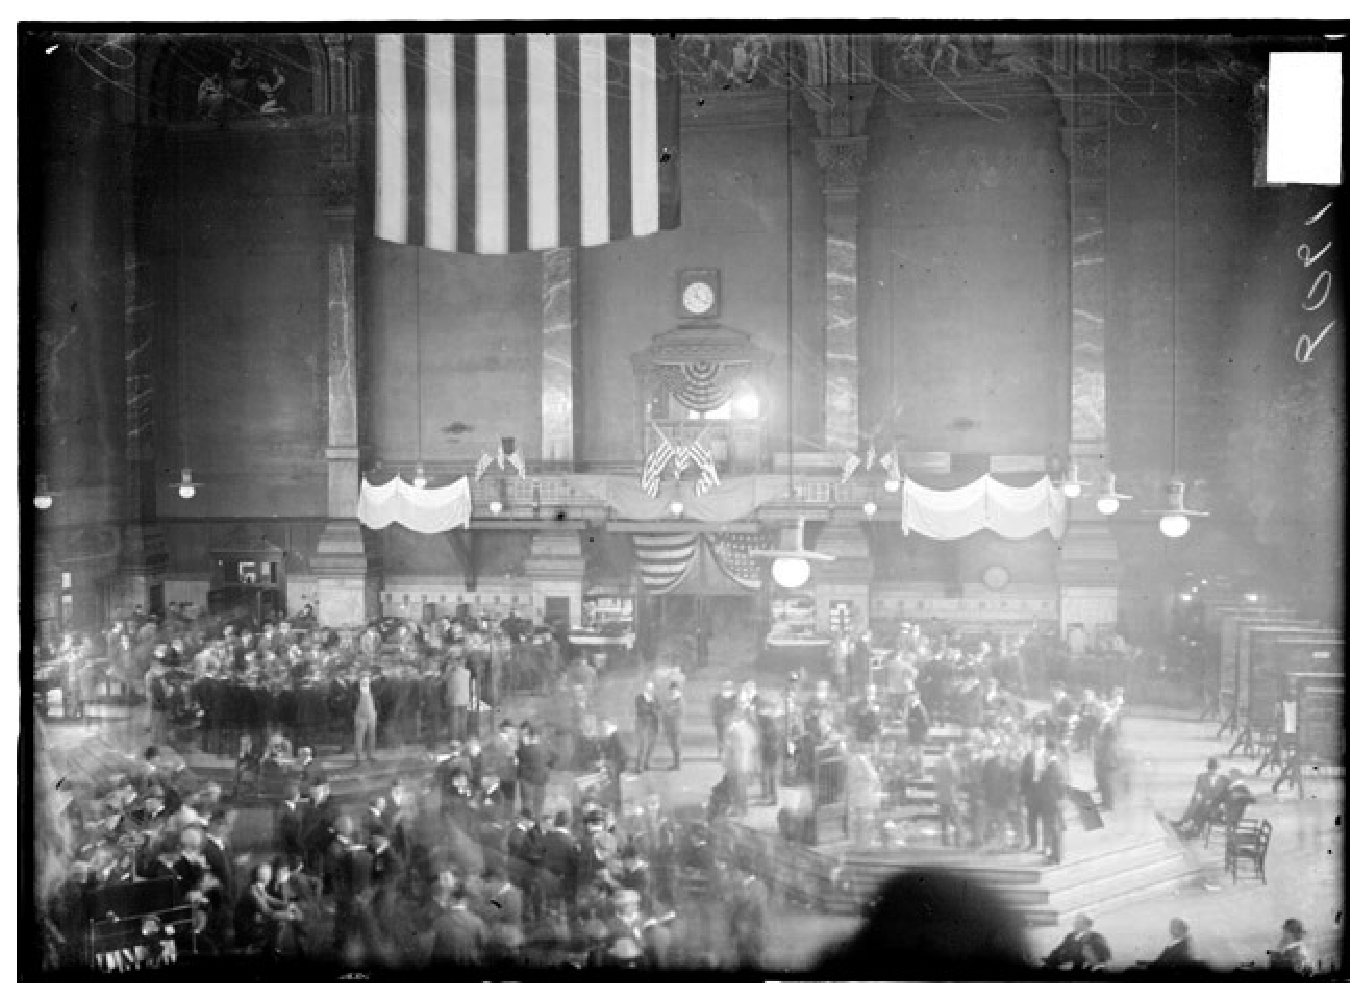
\includegraphics[width=0.9\linewidth]{CBOT}
\end{center}
\caption{Chicago Board of Trade}
\end{wrapfigure}


Beispiele für Derivate:
\begin{itemize}
\item Termingeschäfte: Verträge, bei denen die Erbringung von Leistung und Gegenleistung zu einem zukünftigen Zeitpunkt heute vereinbart werden. Zu Termingeschäften geören:
\begin{enumerate}
\item Warentermingeschäfte
\item Devisentermingeschäfte: z.B. kaufe zum Zeitpunkt $T$ $a$ US Dollar zu einem Wechselkurs von $b$.
\item Finanztermingeschäfte: Man unterscheidet hier Financial Forwards und Financial Futures. Futures werden an Märkten gehandelt, z.B. am CBOT (Chicago Board of Trade). 
\end{enumerate}
\item Optionen: Der Käufer der Option hat das Wahlrecht (aber nicht die Verpflichtung) ein bestimmtes Finanzgut (z.B. eine Aktie) (underlying, underlying asset) bis zu einem zukünftigen Zeitpunkt $T$ (maturity, expiry) zu einem vereinbarten Preis $K$ (strike price, excerise price, Ausübungspreis) zu kaufen oder zu verkaufen. Das Kaufrecht wird Call-Option genannt und dan Verkaufsrecht wird Put-Option genannt. Man unterscheidet:
\begin{itemize}
\item Europäische Option: Ausübung ist nur zum Zeitpunkt $T$ möglich.
\item Amerikanische Aption: Ausübung jederzeit bis zum Zeitpunkt $T$ möglich.
\end{itemize}
\end{itemize}

\begin{beispiel}[Preisbestimmung einer europäischen Call-Option]
Sei $t=0$ der aktuelle Zeitpunkt, $T>0$ der Ausübungszeitpunkt, $(S_t)$ der stochastische Prozess, der den Preis der zugrunde liegenden Aktie beschreibt, und $K$ der Ausübungspreis. Die Auszahlung des Calls zum Zeitpunkt $T$ ist gegeben durch die Funktion 
\[
H \da \max\{0,S_T - K\} = (S_T-K)^+.
\]

Sei der Anfangswert der Aktie $S_0=10\$$. Wir nehmen an, dass die Aktie zum Zeitpunkt $T$ nur zwei Werte annehmen kann: $S_T(\omega_1) = 20\$$, $S_T(\omega_2) = 7,5\$$ mit Wahrscheinlichkeiten $p$ und $1-p$. Sei $K=15\$$. Dann ist die Auszahlung des Calls
\[
H= (S_T-K)^+ = 
\begin{cases}
5, \text{ mit Wahrscheinlichkeit $p$}\\
0, \text{ mit Wahrscheinlichkeit $1-p$}
\end{cases}
\]
Wir nehmen weiter an, dass es als zusätzliche Investitionsmöglichkeit (neben der Aktie) in dem Markt noch ein Bankkonto gibt, mit Zinssatz $r=0$ für Soll- und Habenpositionen. Was ist der Preis $\pi(H)$ für diese Option?

Idee: No-arbitrage-Prinzip: Es darf keine Arbitrage (risikoloser Gewinn) möglich sein. Die Auszahlung $H$ wird mit anderen Finanzinstrumenten (hier Aktie und Bankkonto) repliziert. Das Anfangskapital, das nötig ist, um $H$ zu repräsentieren, ist der Preis der Option. Im Folgenden bezeichnen wir mit $(\alpha, \beta)$ eine Handelsstrategie, wobei $\alpha$ die Anlage in die Aktie (Stückzahl) angibt und $\beta$ ist die Anlage auf dem Bankkonto. Für $\alpha<0$ spricht man vom Leerverkauf. Die Aktien können in belieben Anteilen ge- und verkauft werden. Der Wert des Portfolios aus Aktie und Bankkonto zum Zeitpunkt $t=0$ ist $V_0(\alpha,\beta) = \beta + \alpha\cdot S_0$ und zum Zeitpunk $t=T$ $V_T(\alpha,\beta) = \beta + \alpha \cdot S_T$.

Replizieren der Auszahlung bedeutet nun, dass man $H=V_T(\alpha,\beta)$ setzt, also $\beta + \alpha \cdot S_T(\omega) = H(\omega)$. Dies gibt für $\omega \in \{\omega_1,\omega_2\}$ ein lineares Gleichungssytem mit zwei Gleichungen:
\begin{align*}
\beta + \alpha \cdot 20  &= 5 \\
\beta + \alpha \cdot 7,5  &= 0 
\end{align*}
Lösen nach $\alpha, \beta$ liefert $\alpha=\frac 25$ und $\beta = -3$. Damit ist $V_0(\alpha,\beta) = -3 + \frac25\cdot 10 = 1$. Die replizierende Strategie (Hedging-Strategie) für den Call $H$ ist: Leihe heute 3\$ von der Bank und kaufe $\frac25$ Aktien. Die Gesamtinvestition ist dann 1\$.

Zum Zeitpunkt $T$ gibt es zwei Szenarios:
\begin{enumerate}
\item $S_T=20\$$. Verkauf der Aktien liefert $\frac 25 \cdot 20\$ = 8\$$. Nach der Kreditrückzahlung von $3\$$ bleiben $5\$$.
\item $S_T=7,5\$$. Verkauf der Aktie liefert $\frac 25 \cdot 7,5\$ = 3\$$. Nach der Kreditrückzahlung von $4\$$ bleiben $0\$$.
\end{enumerate}

Angenommen, wir verkaufen einem Kunden die Call-Option zum Preis von $1\$$ und investieren diesen wie oben beschrieben. Im ersten Szenario ($S_T=20$) wird der Kunde die von seinem Recht gebrauch machen und den Call ausüben. Er möchte also die Aktie zum Ausübungspreis $K=15\$$ kaufen. Unsere replizierende Strategie hat uns schon $5\$$ eingebracht, wir bekommen nun noch $K=15\$$ hinzu und können den Marktpreis einer Aktie von $20\$$ bezahlen und sie dem Kunden geben.

Wir haben uns mit der replizierenden Strategie perfekt gegen das Risiko, dass der Kunde  von seinem Ausübungsrecht gebrauch macht, abgesichert (“Hedging”).

Im zweiten Szenario ($S_T=7,5\$$) wird der Kunde den Call nicht ausüben und die Aktie lieber am Markt für $S_T=7,5\$$, als von uns zum Preis $K=15\$$. Unsere replizierende Strategie hat uns $0\$$ eingebracht.

Angenommen, es gelte $\pi(H)>1$: Wir verkaufen Option zum Preis $\pi(H)$ und replizieren sie wie oben mit den Kosten von $1\$$. Der risikolose Gewinn beträgt $\pi(H) - 1$. Nehmen wir statt dessen an, dass $\pi(H)<1$ gilt, dann kaufen wir eine Option zum Preis $\pi(H)$ und verkaufen die replizierende Strategie. Der risikolose Gewinn wäre dann $1-\pi(H)$.

\textbf{Beachte:} $\pi(H)$ ist unabhängig von der Wahrscheinlichkeit $p$ (“real world probability”).
\end{beispiel}

\section{Endliche Finanzmärkte}

Es werden nun endliche Finazmärkte, die durch endlich viele Marktzustände und durch endlich viele Handelszeitpunkte charakterisiert sind, betrachtet. Es sei $J=\{0,1,\ldots,T\}$. Wir betrachten einen filtrierten Wahrscheinlichkeitsraum $(\Omega,\cF,(\cF_t),P)$ mit endlichen $\Omega$ und $\cF=\mathcal P(\Omega)$. Weitere sei $P(\{\omega\})>0$ für alle $\omega\in\Omega$. Handelszeitpunkt seien die Zeitpunkte $t=0,1,\ldots,T$. Der Markt besteht aus $d+1$ Anlagemöglichkeiten: Einer risikolosen Anlagemöglichkeit $B$ (“Bond”) mit determinisitischem Bond-Preis $(B_t)_{t\in I}$, wobei $B_0=1$ und $B_t>0$ für $t=1,\ldots,T$, und $d$ risikobehafteten Anlagemöglichkeiten (“stocks”) mit Preisprozessen $(S_t^k)_{t\in I}$, $k=1,\ldots,d$, wobei $S_t=(S_t^1,\ldots,S_t^d)^\top\in \MdR^d$ und $S_t^k(\omega)>0$ für alle $k=1,\ldots,d$, $t\in I$, $\omega\in \Omega$. Die Prozesse $(S_t^k)_{t\in I}$ sein für alle $k=1,\ldots,d$ adaptiert bezüglich der gegebenen Filtration $(\cF_t)_{t\in I}$.


\setcounter{secnumdepth}{-1}
\chapter{Satz um Satz (hüpft der Has)}
\theoremlisttype{optname}
\listtheorems{satz,beispiel}

\renewcommand{\indexname}{Stichwortverzeichnis}
%\addtocounter{chapter}{1}
%\addcontentsline{toc}{chapter}{\protect\numberline {\thechapter}Stichwortverzeichnis}
\addcontentsline{toc}{chapter}{Stichwortverzeichnis}
\printindex
\end{document}
